% Options for packages loaded elsewhere
\PassOptionsToPackage{unicode}{hyperref}
\PassOptionsToPackage{hyphens}{url}
\PassOptionsToPackage{dvipsnames,svgnames,x11names}{xcolor}
\documentclass[
  italian,
  10pt,
]{book}
\usepackage{xcolor}
\usepackage[papersize={6in,9in},inner=0.75in,outer=0.5in,top=0.7in,bottom=0.7in]{geometry}
\usepackage{amsmath,amssymb}
\setcounter{secnumdepth}{-\maxdimen} % remove section numbering
\usepackage{iftex}
\ifPDFTeX
  \usepackage[T1]{fontenc}
  \usepackage[utf8]{inputenc}
  \usepackage{textcomp} % provide euro and other symbols
\else % if luatex or xetex
  \usepackage{unicode-math} % this also loads fontspec
  \defaultfontfeatures{Scale=MatchLowercase}
  \defaultfontfeatures[\rmfamily]{Ligatures=TeX,Scale=1}
\fi
\usepackage{lmodern}
\ifPDFTeX\else
  % xetex/luatex font selection
\fi
% Use upquote if available, for straight quotes in verbatim environments
\IfFileExists{upquote.sty}{\usepackage{upquote}}{}
\IfFileExists{microtype.sty}{% use microtype if available
  \usepackage[]{microtype}
  \UseMicrotypeSet[protrusion]{basicmath} % disable protrusion for tt fonts
}{}
\makeatletter
\@ifundefined{KOMAClassName}{% if non-KOMA class
  \IfFileExists{parskip.sty}{%
    \usepackage{parskip}
  }{% else
    \setlength{\parindent}{0pt}
    \setlength{\parskip}{6pt plus 2pt minus 1pt}}
}{% if KOMA class
  \KOMAoptions{parskip=half}}
\makeatother
\usepackage{color}
\usepackage{fancyvrb}
\newcommand{\VerbBar}{|}
\newcommand{\VERB}{\Verb[commandchars=\\\{\}]}
\DefineVerbatimEnvironment{Highlighting}{Verbatim}{commandchars=\\\{\}}
% Add ',fontsize=\small' for more characters per line
\usepackage{framed}
\definecolor{shadecolor}{RGB}{248,248,248}
\newenvironment{Shaded}{\begin{snugshade}}{\end{snugshade}}
\newcommand{\AlertTok}[1]{\textcolor[rgb]{0.94,0.16,0.16}{#1}}
\newcommand{\AnnotationTok}[1]{\textcolor[rgb]{0.56,0.35,0.01}{\textbf{\textit{#1}}}}
\newcommand{\AttributeTok}[1]{\textcolor[rgb]{0.13,0.29,0.53}{#1}}
\newcommand{\BaseNTok}[1]{\textcolor[rgb]{0.00,0.00,0.81}{#1}}
\newcommand{\BuiltInTok}[1]{#1}
\newcommand{\CharTok}[1]{\textcolor[rgb]{0.31,0.60,0.02}{#1}}
\newcommand{\CommentTok}[1]{\textcolor[rgb]{0.56,0.35,0.01}{\textit{#1}}}
\newcommand{\CommentVarTok}[1]{\textcolor[rgb]{0.56,0.35,0.01}{\textbf{\textit{#1}}}}
\newcommand{\ConstantTok}[1]{\textcolor[rgb]{0.56,0.35,0.01}{#1}}
\newcommand{\ControlFlowTok}[1]{\textcolor[rgb]{0.13,0.29,0.53}{\textbf{#1}}}
\newcommand{\DataTypeTok}[1]{\textcolor[rgb]{0.13,0.29,0.53}{#1}}
\newcommand{\DecValTok}[1]{\textcolor[rgb]{0.00,0.00,0.81}{#1}}
\newcommand{\DocumentationTok}[1]{\textcolor[rgb]{0.56,0.35,0.01}{\textbf{\textit{#1}}}}
\newcommand{\ErrorTok}[1]{\textcolor[rgb]{0.64,0.00,0.00}{\textbf{#1}}}
\newcommand{\ExtensionTok}[1]{#1}
\newcommand{\FloatTok}[1]{\textcolor[rgb]{0.00,0.00,0.81}{#1}}
\newcommand{\FunctionTok}[1]{\textcolor[rgb]{0.13,0.29,0.53}{\textbf{#1}}}
\newcommand{\ImportTok}[1]{#1}
\newcommand{\InformationTok}[1]{\textcolor[rgb]{0.56,0.35,0.01}{\textbf{\textit{#1}}}}
\newcommand{\KeywordTok}[1]{\textcolor[rgb]{0.13,0.29,0.53}{\textbf{#1}}}
\newcommand{\NormalTok}[1]{#1}
\newcommand{\OperatorTok}[1]{\textcolor[rgb]{0.81,0.36,0.00}{\textbf{#1}}}
\newcommand{\OtherTok}[1]{\textcolor[rgb]{0.56,0.35,0.01}{#1}}
\newcommand{\PreprocessorTok}[1]{\textcolor[rgb]{0.56,0.35,0.01}{\textit{#1}}}
\newcommand{\RegionMarkerTok}[1]{#1}
\newcommand{\SpecialCharTok}[1]{\textcolor[rgb]{0.81,0.36,0.00}{\textbf{#1}}}
\newcommand{\SpecialStringTok}[1]{\textcolor[rgb]{0.31,0.60,0.02}{#1}}
\newcommand{\StringTok}[1]{\textcolor[rgb]{0.31,0.60,0.02}{#1}}
\newcommand{\VariableTok}[1]{\textcolor[rgb]{0.00,0.00,0.00}{#1}}
\newcommand{\VerbatimStringTok}[1]{\textcolor[rgb]{0.31,0.60,0.02}{#1}}
\newcommand{\WarningTok}[1]{\textcolor[rgb]{0.56,0.35,0.01}{\textbf{\textit{#1}}}}
\usepackage{longtable,booktabs,array}
\usepackage{caption}
\captionsetup[table]{skip=6pt}
\newcounter{none} % for unnumbered tables
\usepackage{calc} % for calculating minipage widths
% Correct order of tables after \paragraph or \subparagraph
\usepackage{etoolbox}
\makeatletter
\patchcmd\longtable{\par}{\if@noskipsec\mbox{}\fi\par}{}{}
\makeatother
\usepackage{graphicx}
\makeatletter
\newsavebox\pandoc@box
\newcommand*\pandocbounded[1]{% scales image to fit in text height/width
  \sbox\pandoc@box{#1}%
  \Gscale@div\@tempa{\textheight}{\dimexpr\ht\pandoc@box+\dp\pandoc@box\relax}%
  \Gscale@div\@tempb{\linewidth}{\wd\pandoc@box}%
  \ifdim\@tempb\p@<\@tempa\p@\let\@tempa\@tempb\fi% select the smaller of both
  \ifdim\@tempa\p@<\p@\scalebox{\@tempa}{\usebox\pandoc@box}%
  \else\usebox{\pandoc@box}%
  \fi%
}
% Set default figure placement to htbp
\def\fps@figure{htbp}
\makeatother
\ifLuaTeX
\usepackage[bidi=basic,shorthands=off]{babel}
\else
\usepackage[bidi=default,shorthands=off]{babel}
\fi
\ifLuaTeX
  \usepackage{selnolig} % disable illegal ligatures
\fi
\setlength{\emergencystretch}{3em} % prevent overfull lines
\providecommand{\tightlist}{%
  \setlength{\itemsep}{0pt}\setlength{\parskip}{0pt}}
\usepackage{fvextra}
\usepackage{float}
\usepackage{xurl}
\usepackage[htt]{hyphenat}
\DefineVerbatimEnvironment{Highlighting}{Verbatim}{breaklines,breakanywhere,fontsize=\small,commandchars=\\\{\}}
\floatplacement{figure}{H}
\setlength{\emergencystretch}{8em}
\sloppy
\usepackage{bookmark}
\IfFileExists{xurl.sty}{\usepackage{xurl}}{} % add URL line breaks if available
\urlstyle{same}
% fallback for those not using the hyperref driver hyperxmp:
\makeatletter
\@ifundefined{xmpquote}{\newcommand{\xmpquote}[1]{#1}}{}
\makeatother
\hypersetup{
  pdftitle={Quaderno AI},
  pdfauthor={Andrea Merlin},
  pdflang={it},
  colorlinks=true,
  linkcolor={blue},
  filecolor={Maroon},
  citecolor={Blue},
  urlcolor={blue},
  pdfcreator={LaTeX via pandoc}}

\title{Quaderno AI}
\usepackage{etoolbox}
\makeatletter
\providecommand{\subtitle}[1]{% add subtitle to \maketitle
  \apptocmd{\@title}{\par {\large #1 \par}}{}{}
}
\makeatother
\subtitle{Concetti, strumenti e percorsi pratici per lo sviluppo
software con AI}
\author{Andrea Merlin}
\date{Numero 1 - Novembre 2026}

\begin{document}
\frontmatter
\maketitle

{
\setcounter{tocdepth}{1}
\tableofcontents
}
\mainmatter
\chapter{Capitolo 2}\label{capitolo-2}

\section{Un MCP Server con Entity Framework Core: dati, query e
primitivi
avanzati}\label{un-mcp-server-con-entity-framework-core-dati-query-e-primitivi-avanzati}

\textbf{Abstract.} Nel primo capitolo abbiamo costruito server MCP che
espongono tool ``senza memoria'': file system e chiamate HTTP. Ora
facciamo il passo successivo: un server che parla con un
\textbf{database relazionale} tramite \textbf{Entity Framework Core}, il
framework ORM di .NET. Implementeremo un catalogo prodotti completo ---
letture, ricerche, inserimenti, aggiornamenti e cancellazioni ---
scopriremo il pattern giusto per usare un \texttt{DbContext} dentro un
tool, affronteremo le migrazioni e i trasporti \texttt{stdio} e HTTP, e
infine vedremo come un tool può comunicare il proprio avanzamento con il
primitivo \textbf{Progress}.

\subsection{Cosa imparerai in questo
capitolo}\label{cosa-imparerai-in-questo-capitolo}

Al termine della lettura e della pratica saprai:

\begin{itemize}
\tightlist
\item
  spiegare perché un agente ha bisogno di \textbf{dati persistenti} e
  come un MCP server può fornirglieli;
\item
  usare \textbf{Entity Framework Core 10} per modellare entità e
  relazioni;
\item
  collegare un \texttt{DbContext} a un tool MCP con il pattern
  \textbf{\texttt{IDbContextFactory}}, evitando i problemi di lifetime;
\item
  creare il database con \texttt{EnsureCreated} e, per i progetti reali,
  con le \textbf{migrazioni} (\texttt{dotnet\ ef});
\item
  implementare tool di \textbf{lettura} e \textbf{scrittura} con query
  LINQ, filtri e gestione degli errori;
\item
  esporre lo stesso server su \textbf{\texttt{stdio}} e su
  \textbf{HTTP};
\item
  usare il primitivo \textbf{Progress} per comunicare l'avanzamento di
  un tool.
\end{itemize}

\subsection{Prerequisiti}\label{prerequisiti}

\begin{itemize}
\tightlist
\item
  Aver letto (o padroneggiare) il Capitolo 1: in particolare tool,
  trasporti, configurazione dei client e MCP Inspector;
\item
  .NET SDK 10 e un editor (VS Code, Visual Studio o Rider);
\item
  conoscenza di base del linguaggio \textbf{LINQ} e, facoltativamente,
  di SQL.
\end{itemize}

\subsection{Convenzioni}\label{convenzioni}

Valgono le convenzioni del Capitolo 1. In più, in questo capitolo
useremo \textbf{SQLite} come database: è un database relazionale
completo, basato su file, che non richiede alcun server da installare
--- perfetto per un server \texttt{stdio} locale. I concetti e il codice
si trasferiscono quasi identici a SQL Server o PostgreSQL, cambiando
solo il provider (lo vedremo).

Come nel capitolo precedente, ogni frammento è stato \textbf{compilato
ed eseguito} con .NET 10, \texttt{ModelContextProtocol} 2.3.0 ed Entity
Framework Core 10.0.14.

\section{2.1 Perché un database in un MCP
server}\label{perchuxe9-un-database-in-un-mcp-server}

Nel Capitolo 1 i nostri server erano ``senza stato'': il server del file
system leggeva e scriveva file, quello meteo interrogava un'API esterna,
ma nessuno \textbf{ricordava} nulla tra una chiamata e l'altra. In
moltissimi scenari reali, però, l'agente ha bisogno di dati che
\textbf{persistono}, si \textbf{interrogano} e si \textbf{aggregano}.

\subsection{2.1.1 Cosa chiede un agente a un
database}\label{cosa-chiede-un-agente-a-un-database}

Pensa a un assistente aziendale. Le sue richieste tipiche sono:

\begin{itemize}
\tightlist
\item
  ``Quanti ordini sono stati evasi la settimana scorsa?'' --- una
  \textbf{aggregazione};
\item
  ``Trovami i clienti che non comprano da più di sei mesi'' --- una
  \textbf{query con filtro};
\item
  ``Aggiungi questo prodotto al catalogo con prezzo 29,90'' --- una
  \textbf{scrittura};
\item
  ``Quali sono le categorie più vendute?'' --- una \textbf{join} con
  raggruppamento.
\end{itemize}

Nessuna di queste operazioni è ragionevolmente realizzabile leggendo
file di testo o chiamando API generiche: serve un \textbf{motore di
interrogazione}, e un database relazionale è lo strumento naturale.

\subsection{2.1.2 Il ruolo del MCP
server}\label{il-ruolo-del-mcp-server}

Il MCP server si colloca esattamente nel punto giusto: è il
\textbf{ponte} tra il modello e il database. Da un lato espone
\emph{tool} descrittivi (\texttt{list\_products},
\texttt{create\_product}, \ldots) che il modello scopre e invoca;
dall'altro traduce quei tool in \textbf{query SQL} (o, meglio, in query
LINQ che il provider traduce in SQL) e restituisce risultati
strutturati.

Il modello non sa nulla di tabelle, indici o join: vede un menu di
strumenti ben descritti. Il database non sa nulla di modelli o di
prompt: riceve query. Il server è il traduttore che vive in mezzo, e il
suo compito è rendere l'incontro \textbf{sicuro, controllato e
coerente}.

\subsection{2.1.3 Perché Entity Framework
Core}\label{perchuxe9-entity-framework-core}

Potremmo usare ADO.NET o un micro-ORM come Dapper per scrivere SQL a
mano. Ma Entity Framework Core offre tre vantaggi decisivi per questo
scenario:

\begin{enumerate}
\def\labelenumi{\arabic{enumi}.}
\tightlist
\item
  \textbf{Modello a oggetti.} Definiamo entità C\# (\texttt{Product},
  \texttt{Category}) e relazioni; EF Core si occupa dello schema e delle
  query.
\item
  \textbf{LINQ.} Le query si scrivono in C\# tipizzato, con il
  completamento automatico e il controllo dei tipi a compile time.
\item
  \textbf{Provider multipli.} Lo stesso codice funziona con SQLite, SQL
  Server, PostgreSQL, MySQL e altri, cambiando un solo pacchetto e una
  stringa di connessione.
\end{enumerate}

In più, EF Core è il modo \textbf{idiomatico} di accedere ai dati in
.NET: un lettore che conosce ASP.NET Core troverà naturale integrare un
\texttt{DbContext} in un server MCP.

\subsection{2.1.4 La sfida specifica di MCP: il lifetime del
DbContext}\label{la-sfida-specifica-di-mcp-il-lifetime-del-dbcontext}

C'è una complicazione, ed è il motivo per cui questo capitolo esiste: un
\texttt{DbContext} è progettato per vivere \textbf{poco}, legato a una
singola unità di lavoro. In una richiesta web, per esempio, vive per la
durata della richiesta. In un server MCP, invece, ogni invocazione di
tool è un ``lavoro'' a sé, e il server resta in vita a lungo.

Se iniettassimo un singolo \texttt{DbContext} condiviso tra tutte le
invocazioni, incapperemmo in problemi classici: contesto non
thread-safe, tracking che cresce senza controllo, dati stantii. La
soluzione corretta --- che esploreremo e useremo --- è il
\textbf{\texttt{IDbContextFactory\textless{}T\textgreater{}}}: una
factory che crea un contesto nuovo per ogni invocazione. Dedichiamo a
questo pattern un'intera sezione, perché è il cuore dell'integrazione
tra EF Core e MCP.

\subsection{2.1.5 La mappa del capitolo}\label{la-mappa-del-capitolo}

Partiremo da un ripasso essenziale di EF Core, poi definiremo il dominio
di esempio (un catalogo prodotti), creeremo il progetto, i modelli e il
database. Implementeremo i tool di lettura e scrittura, li esporremo su
\texttt{stdio} e HTTP, e infine vedremo come comunicare il progresso di
un'operazione. Alla fine avrai un server MCP \textbf{con persistenza}
completo, pronto per essere collegato a Claude Desktop o VS Code.

\section{2.2 Entity Framework Core in
sintesi}\label{entity-framework-core-in-sintesi}

Prima di scrivere codice, ripassiamo i concetti essenziali di Entity
Framework Core. Se lo conosci già, puoi scorrere velocemente: serve solo
ad allineare il vocabolario.

\subsection{2.2.1 Cos'è un ORM}\label{cosuxe8-un-orm}

Entity Framework Core è un \textbf{Object-Relational Mapper} (ORM): una
libreria che mappa le \textbf{entità} C\# (classi) sulle
\textbf{tabelle} del database e le \textbf{proprietà} sulle
\textbf{colonne}. Il programmatore lavora con oggetti e LINQ; l'ORM
traduce il tutto in SQL e materializza i risultati in oggetti.

Il punto di ingresso è il \textbf{\texttt{DbContext}}: una classe che
rappresenta una sessione di lavoro con il database. Contiene un
\texttt{DbSet\textless{}T\textgreater{}} per ogni entità e permette di
eseguire query, inserimenti, aggiornamenti e cancellazioni, coordinati
dal metodo \texttt{SaveChanges()}.

\subsection{2.2.2 Le entità}\label{le-entituxe0}

Un'entità è una semplice classe C\# con proprietà pubbliche. Per
convenzione, la proprietà \texttt{Id} (o
\texttt{\textless{}NomeClasse\textgreater{}Id}) viene riconosciuta come
\textbf{chiave primaria}:

\begin{Shaded}
\begin{Highlighting}[]
\KeywordTok{public} \KeywordTok{sealed} \KeywordTok{class}\NormalTok{ Category}
\OperatorTok{\{}
    \KeywordTok{public} \DataTypeTok{int}\NormalTok{ Id }\OperatorTok{\{} \KeywordTok{get}\OperatorTok{;} \KeywordTok{set}\OperatorTok{;} \OperatorTok{\}}
    \KeywordTok{public}\NormalTok{ required }\DataTypeTok{string}\NormalTok{ Name }\OperatorTok{\{} \KeywordTok{get}\OperatorTok{;} \KeywordTok{set}\OperatorTok{;} \OperatorTok{\}}
    \KeywordTok{public}\NormalTok{ List}\OperatorTok{\textless{}}\NormalTok{Product}\OperatorTok{\textgreater{}}\NormalTok{ Products }\OperatorTok{\{} \KeywordTok{get}\OperatorTok{;} \KeywordTok{set}\OperatorTok{;} \OperatorTok{\}} \OperatorTok{=} \OperatorTok{[];}
\OperatorTok{\}}
\end{Highlighting}
\end{Shaded}

La proprietà \texttt{Products} è una \textbf{navigation property}:
rappresenta la relazione ``una categoria ha molti prodotti''. EF Core la
userà per eseguire le join quando serve.

\subsection{2.2.3 Il DbContext}\label{il-dbcontext}

La classe \texttt{DbContext} dichiara quali entità fanno parte del
modello:

\begin{Shaded}
\begin{Highlighting}[]
\KeywordTok{public} \KeywordTok{sealed} \KeywordTok{class} \FunctionTok{CatalogDbContext}\OperatorTok{(}\NormalTok{DbContextOptions}\OperatorTok{\textless{}}\NormalTok{CatalogDbContext}\OperatorTok{\textgreater{}}\NormalTok{ options}\OperatorTok{)}
    \OperatorTok{:} \FunctionTok{DbContext}\OperatorTok{(}\NormalTok{options}\OperatorTok{)}
\OperatorTok{\{}
    \KeywordTok{public}\NormalTok{ DbSet}\OperatorTok{\textless{}}\NormalTok{Category}\OperatorTok{\textgreater{}}\NormalTok{ Categories }\OperatorTok{=\textgreater{}}\NormalTok{ Set}\OperatorTok{\textless{}}\NormalTok{Category}\OperatorTok{\textgreater{}();}
    \KeywordTok{public}\NormalTok{ DbSet}\OperatorTok{\textless{}}\NormalTok{Product}\OperatorTok{\textgreater{}}\NormalTok{ Products }\OperatorTok{=\textgreater{}}\NormalTok{ Set}\OperatorTok{\textless{}}\NormalTok{Product}\OperatorTok{\textgreater{}();}
\OperatorTok{\}}
\end{Highlighting}
\end{Shaded}

Il costruttore primario riceve
\texttt{DbContextOptions\textless{}T\textgreater{}}, che contiene la
configurazione (provider, stringa di connessione) e che verrà fornita
dal sistema di dependency injection.

\subsection{2.2.4 Le query LINQ}\label{le-query-linq}

EF Core traduce le query LINQ in SQL. Un esempio:

\begin{Shaded}
\begin{Highlighting}[]
\DataTypeTok{var}\NormalTok{ books }\OperatorTok{=}\NormalTok{ await db}\OperatorTok{.}\FunctionTok{Products}
    \OperatorTok{.}\FunctionTok{Where}\OperatorTok{(}\NormalTok{p }\OperatorTok{=\textgreater{}}\NormalTok{ p}\OperatorTok{.}\FunctionTok{Category}\OperatorTok{!.}\FunctionTok{Name} \OperatorTok{==} \StringTok{"Books"}\OperatorTok{)}
    \OperatorTok{.}\FunctionTok{OrderBy}\OperatorTok{(}\NormalTok{p }\OperatorTok{=\textgreater{}}\NormalTok{ p}\OperatorTok{.}\FunctionTok{Name}\OperatorTok{)}
    \OperatorTok{.}\FunctionTok{ToListAsync}\OperatorTok{();}
\end{Highlighting}
\end{Shaded}

L'esecuzione avviene \textbf{solo quando si materializza la query} (con
\texttt{ToListAsync}, \texttt{ToArrayAsync},
\texttt{FirstOrDefaultAsync}, ecc.): fino a quel momento si compone un
albero di espressioni che il provider traduce. Questo dettaglio è
importante perché ci permette di costruire query \textbf{condizionali},
aggiungendo filtri solo se necessari.

\subsection{2.2.5 Le operazioni di
scrittura}\label{le-operazioni-di-scrittura}

Le scritture passano dal \emph{change tracker} di EF Core:

\begin{Shaded}
\begin{Highlighting}[]
\NormalTok{db}\OperatorTok{.}\FunctionTok{Products}\OperatorTok{.}\FunctionTok{Add}\OperatorTok{(}\KeywordTok{new}\NormalTok{ Product }\OperatorTok{\{}\NormalTok{ Name }\OperatorTok{=} \StringTok{"Headphones"}\OperatorTok{,}\NormalTok{ Price }\OperatorTok{=} \FloatTok{199.99m}\OperatorTok{,}\NormalTok{ CategoryId }\OperatorTok{=} \DecValTok{1} \OperatorTok{\});}
\NormalTok{await db}\OperatorTok{.}\FunctionTok{SaveChangesAsync}\OperatorTok{();} \CommentTok{// genera INSERT}
\end{Highlighting}
\end{Shaded}

\texttt{SaveChanges()} rileva le modifiche (aggiunte, modifiche,
cancellazioni) e le applica al database in una \textbf{transazione
implicita}.

\subsection{2.2.6 I provider}\label{i-provider}

EF Core separa il nucleo dai \textbf{provider}, uno per database. I più
usati:

\begin{itemize}
\tightlist
\item
  \textbf{SQLite:} \texttt{Microsoft.EntityFrameworkCore.Sqlite}, adatto
  allo sviluppo locale e a database su file.
\item
  \textbf{SQL Server:} \texttt{Microsoft.EntityFrameworkCore.SqlServer},
  usato spesso in ambienti Windows e Azure.
\item
  \textbf{PostgreSQL:} \texttt{Npgsql.EntityFrameworkCore.PostgreSQL},
  provider open source.
\item
  \textbf{InMemory:} \texttt{Microsoft.EntityFrameworkCore.InMemory},
  utile per alcuni test ma non equivalente a un vero database
  relazionale.
\end{itemize}

In questo capitolo useremo \textbf{SQLite} per la sua semplicità
operativa: zero installazioni, un solo file. Alla fine del capitolo
vedremo come passare a un altro provider cambiando poco più di una riga.

\subsection{2.2.7 La configurazione tramite
DI}\label{la-configurazione-tramite-di}

In un'applicazione .NET moderna, il \texttt{DbContext} si registra nel
container di dependency injection. EF Core offre due modalità:

\begin{itemize}
\tightlist
\item
  \texttt{AddDbContext\textless{}T\textgreater{}} --- registra un
  contesto \textbf{scoped} (condiviso nell'ambito di una richiesta);
\item
  \texttt{AddDbContextFactory\textless{}T\textgreater{}} --- registra
  una \textbf{factory} che crea un contesto nuovo a richiesta.
\end{itemize}

Come anticipato, per i tool MCP useremo
\texttt{AddDbContextFactory\textless{}T\textgreater{}}: ogni invocazione
di tool avrà il suo contesto fresco, senza conflitti e senza tracking
accumulato. Ne vedremo i dettagli operativi nella sezione dedicata.

\section{2.3 Il dominio di esempio: un catalogo
prodotti}\label{il-dominio-di-esempio-un-catalogo-prodotti}

Per tutto il capitolo lavoreremo su un dominio semplice ma realistico:
un \textbf{catalogo prodotti} organizzato in \textbf{categorie}. Due
entità, una relazione, e un insieme di operazioni che coprono tutti i
casi tipici: lettura con filtro, creazione, cancellazione.

\subsection{2.3.1 Il modello concettuale}\label{il-modello-concettuale}

\begin{itemize}
\tightlist
\item
  \textbf{Category} --- una categoria di prodotti (per esempio
  ``Books'', ``Electronics''). Ha un nome univoco.
\item
  \textbf{Product} --- un prodotto che appartiene a \textbf{una}
  categoria. Ha nome, prezzo e un riferimento alla categoria.
\end{itemize}

La relazione è \textbf{uno-a-molti}: una categoria ha molti prodotti,
ogni prodotto ha una sola categoria.

\begin{figure}
\centering
\pandocbounded{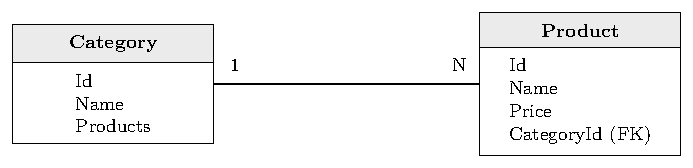
\includegraphics[keepaspectratio,alt={Relazione
uno-a-molti tra Category e Product}]{figure/modello-dati.pdf}}
\caption{Relazione uno-a-molti tra \protect\texttt{Category} e
\protect\texttt{Product}}
\end{figure}

\subsection{2.3.2 Le entità C\#}\label{le-entituxe0-c}

Traduciamo il modello in classi. Nota l'uso di \texttt{required} (C\#
11+) per rendere obbligatorie le proprietà non nullable, e della
collection expression \texttt{{[}{]}} per inizializzare la navigation:

\begin{Shaded}
\begin{Highlighting}[]
\KeywordTok{public} \KeywordTok{sealed} \KeywordTok{class}\NormalTok{ Category}
\OperatorTok{\{}
    \KeywordTok{public} \DataTypeTok{int}\NormalTok{ Id }\OperatorTok{\{} \KeywordTok{get}\OperatorTok{;} \KeywordTok{set}\OperatorTok{;} \OperatorTok{\}}
    \KeywordTok{public}\NormalTok{ required }\DataTypeTok{string}\NormalTok{ Name }\OperatorTok{\{} \KeywordTok{get}\OperatorTok{;} \KeywordTok{set}\OperatorTok{;} \OperatorTok{\}}
    \KeywordTok{public}\NormalTok{ List}\OperatorTok{\textless{}}\NormalTok{Product}\OperatorTok{\textgreater{}}\NormalTok{ Products }\OperatorTok{\{} \KeywordTok{get}\OperatorTok{;} \KeywordTok{set}\OperatorTok{;} \OperatorTok{\}} \OperatorTok{=} \OperatorTok{[];}
\OperatorTok{\}}

\KeywordTok{public} \KeywordTok{sealed} \KeywordTok{class}\NormalTok{ Product}
\OperatorTok{\{}
    \KeywordTok{public} \DataTypeTok{int}\NormalTok{ Id }\OperatorTok{\{} \KeywordTok{get}\OperatorTok{;} \KeywordTok{set}\OperatorTok{;} \OperatorTok{\}}
    \KeywordTok{public}\NormalTok{ required }\DataTypeTok{string}\NormalTok{ Name }\OperatorTok{\{} \KeywordTok{get}\OperatorTok{;} \KeywordTok{set}\OperatorTok{;} \OperatorTok{\}}
    \KeywordTok{public} \DataTypeTok{decimal}\NormalTok{ Price }\OperatorTok{\{} \KeywordTok{get}\OperatorTok{;} \KeywordTok{set}\OperatorTok{;} \OperatorTok{\}}
    \KeywordTok{public} \DataTypeTok{int}\NormalTok{ CategoryId }\OperatorTok{\{} \KeywordTok{get}\OperatorTok{;} \KeywordTok{set}\OperatorTok{;} \OperatorTok{\}}
    \KeywordTok{public}\NormalTok{ Category}\OperatorTok{?}\NormalTok{ Category }\OperatorTok{\{} \KeywordTok{get}\OperatorTok{;} \KeywordTok{set}\OperatorTok{;} \OperatorTok{\}}
\OperatorTok{\}}
\end{Highlighting}
\end{Shaded}

Alcune osservazioni:

\begin{itemize}
\tightlist
\item
  \texttt{Id} è la chiave primaria per convenzione.
\item
  \texttt{Product.CategoryId} è la \textbf{chiave esterna}: EF Core la
  riconosce per convenzione (nome \texttt{Category} + \texttt{Id}) e la
  userà per la relazione.
\item
  \texttt{Product.Category} è la navigation verso il ``lato uno'';
  \texttt{Category.Products} verso il ``lato molti''. Entrambe servono
  per scrivere query leggibili con \texttt{Include}.
\end{itemize}

\subsection{2.3.3 Cosa esporremo come
tool}\label{cosa-esporremo-come-tool}

Dal modello deriviamo un set di tool MCP sensato:

{\def\LTcaptype{none} % do not increment counter
\begin{longtable}[]{@{}
  >{\raggedright\arraybackslash}p{(\linewidth - 4\tabcolsep) * \real{0.2400}}
  >{\raggedright\arraybackslash}p{(\linewidth - 4\tabcolsep) * \real{0.2400}}
  >{\raggedright\arraybackslash}p{(\linewidth - 4\tabcolsep) * \real{0.5200}}@{}}
\toprule\noalign{}
\begin{minipage}[b]{\linewidth}\raggedright
Tool
\end{minipage} & \begin{minipage}[b]{\linewidth}\raggedright
Tipo
\end{minipage} & \begin{minipage}[b]{\linewidth}\raggedright
Descrizione
\end{minipage} \\
\midrule\noalign{}
\endhead
\bottomrule\noalign{}
\endlastfoot
\texttt{list\_products} & Lettura & Elenca i prodotti, con filtro
opzionale per categoria \\
\texttt{search\_products} & Lettura & Cerca prodotti per nome
(sottostringa) \\
\texttt{get\_product} & Lettura & Restituisce un singolo prodotto per
id \\
\texttt{create\_product} & Scrittura & Crea un prodotto in una
categoria \\
\texttt{update\_price} & Scrittura & Aggiorna il prezzo di un
prodotto \\
\texttt{delete\_product} & Scrittura (distruttiva) & Elimina un prodotto
per id \\
\end{longtable}
}

A questi aggiungeremo, nella sezione sul Progress, un tool dimostrativo
per comunicare l'avanzamento di un'operazione.

\subsection{2.3.4 Il tipo di ritorno: un
DTO}\label{il-tipo-di-ritorno-un-dto}

Per le letture non restituiremo le entità EF Core ``grezze'': le
proietteremo in un \textbf{DTO} (Data Transfer Object) con LINQ
\texttt{Select}. Così controlliamo esattamente cosa viaggia verso il
modello, evitando di serializzare navigation property potenzialmente
cicliche (una categoria che contiene i suoi prodotti, che contengono la
categoria\ldots) e dati non necessari:

\begin{Shaded}
\begin{Highlighting}[]
\KeywordTok{public} \KeywordTok{sealed}\NormalTok{ record }\FunctionTok{ProductDto}\OperatorTok{(}\DataTypeTok{int}\NormalTok{ Id}\OperatorTok{,} \DataTypeTok{string}\NormalTok{ Name}\OperatorTok{,} \DataTypeTok{decimal}\NormalTok{ Price}\OperatorTok{,} \DataTypeTok{string}\NormalTok{ Category}\OperatorTok{);}
\end{Highlighting}
\end{Shaded}

Il DTO è un \texttt{record} immutabile: pulito, serializzabile e facile
da leggere. Il nome della categoria viene ``appiattito'' nel DTO, così
il modello riceve già il dato pronto.

\subsection{2.3.5 Il principio guida del
capitolo}\label{il-principio-guida-del-capitolo}

Tutto il codice che segue ruota attorno a un'idea: \textbf{il database
resta nascosto dietro i tool}. Il modello non sa che c'è una tabella
\texttt{Products}; sa che c'è un tool \texttt{list\_products} con un
parametro \texttt{category}. Il server decide quali query eseguire, come
validare gli input e quali errori restituire. Questa separazione è ciò
che rende l'integrazione sicura e manutenibile.

\section{2.4 Setup del progetto e
pacchetti}\label{setup-del-progetto-e-pacchetti}

Prepariamo l'ambiente. Il procedimento ricalca il Capitolo 1, con
l'aggiunta dei pacchetti EF Core.

\subsection{2.4.1 Creare il progetto}\label{creare-il-progetto}

Come per ogni server \texttt{stdio}, partiamo da un progetto console:

\begin{Shaded}
\begin{Highlighting}[]
\OperatorTok{\textgreater{}}\NormalTok{ mkdir }\ExtensionTok{CatalogMcpServer}
\OperatorTok{\textgreater{}}\NormalTok{ cd }\ExtensionTok{CatalogMcpServer}
\OperatorTok{\textgreater{}}\NormalTok{ dotnet }\ExtensionTok{new}\NormalTok{ console }\AttributeTok{{-}n}\NormalTok{ CatalogMcpServer }\AttributeTok{{-}o}\NormalTok{ .}
\end{Highlighting}
\end{Shaded}

\subsection{2.4.2 Aggiungere i pacchetti}\label{aggiungere-i-pacchetti}

Servono quattro pacchetti:

\begin{Shaded}
\begin{Highlighting}[]
\OperatorTok{\textgreater{}}\NormalTok{ dotnet }\ExtensionTok{add}\NormalTok{ package ModelContextProtocol }\AttributeTok{{-}{-}version}\NormalTok{ 2.3.0}
\OperatorTok{\textgreater{}}\NormalTok{ dotnet }\ExtensionTok{add}\NormalTok{ package Microsoft.Extensions.Hosting}
\OperatorTok{\textgreater{}}\NormalTok{ dotnet }\ExtensionTok{add}\NormalTok{ package Microsoft.EntityFrameworkCore.Sqlite }\AttributeTok{{-}{-}version}\NormalTok{ 10.0.14}
\OperatorTok{\textgreater{}}\NormalTok{ dotnet }\ExtensionTok{add}\NormalTok{ package Microsoft.EntityFrameworkCore.Design }\AttributeTok{{-}{-}version}\NormalTok{ 10.0.14}
\end{Highlighting}
\end{Shaded}

A cosa serve ciascuno:

\begin{itemize}
\tightlist
\item
  \texttt{ModelContextProtocol} --- il C\# SDK di MCP (con le estensioni
  DI);
\item
  \texttt{Microsoft.Extensions.Hosting} --- l'host generico
  (\texttt{Host.CreateApplicationBuilder}) per il server \texttt{stdio};
\item
  \texttt{Microsoft.EntityFrameworkCore.Sqlite} --- il provider EF Core
  per SQLite;
\item
  \texttt{Microsoft.EntityFrameworkCore.Design} --- gli strumenti di
  design-time, necessari per il comando \texttt{dotnet\ ef}
  (migrazioni). Si usa solo in sviluppo: per questo, se preferisci, puoi
  marcarlo con \texttt{PrivateAssets="all"}, ma non è indispensabile.
\end{itemize}

\subsection{2.4.3 Il file di progetto
risultante}\label{il-file-di-progetto-risultante}

Dopo l'aggiunta, il file \texttt{CatalogMcpServer.csproj} assomiglierà
a:

\begin{Shaded}
\begin{Highlighting}[]
\NormalTok{\textless{}}\KeywordTok{Project} \OtherTok{Sdk=}\StringTok{"Microsoft.NET.Sdk"}\NormalTok{\textgreater{}}

\NormalTok{  \textless{}}\KeywordTok{PropertyGroup}\NormalTok{\textgreater{}}
\NormalTok{    \textless{}}\KeywordTok{OutputType}\NormalTok{\textgreater{}Exe\textless{}/}\KeywordTok{OutputType}\NormalTok{\textgreater{}}
\NormalTok{    \textless{}}\KeywordTok{TargetFramework}\NormalTok{\textgreater{}net10.0\textless{}/}\KeywordTok{TargetFramework}\NormalTok{\textgreater{}}
\NormalTok{    \textless{}}\KeywordTok{ImplicitUsings}\NormalTok{\textgreater{}enable\textless{}/}\KeywordTok{ImplicitUsings}\NormalTok{\textgreater{}}
\NormalTok{    \textless{}}\KeywordTok{Nullable}\NormalTok{\textgreater{}enable\textless{}/}\KeywordTok{Nullable}\NormalTok{\textgreater{}}
\NormalTok{  \textless{}/}\KeywordTok{PropertyGroup}\NormalTok{\textgreater{}}

\NormalTok{  \textless{}}\KeywordTok{ItemGroup}\NormalTok{\textgreater{}}
\NormalTok{    \textless{}}\KeywordTok{PackageReference} \OtherTok{Include=}\StringTok{"Microsoft.EntityFrameworkCore.Design"} \OtherTok{Version=}\StringTok{"10.0.14"}\NormalTok{ /\textgreater{}}
\NormalTok{    \textless{}}\KeywordTok{PackageReference} \OtherTok{Include=}\StringTok{"Microsoft.EntityFrameworkCore.Sqlite"} \OtherTok{Version=}\StringTok{"10.0.14"}\NormalTok{ /\textgreater{}}
\NormalTok{    \textless{}}\KeywordTok{PackageReference} \OtherTok{Include=}\StringTok{"Microsoft.Extensions.Hosting"} \OtherTok{Version=}\StringTok{"10.0.13"}\NormalTok{ /\textgreater{}}
\NormalTok{    \textless{}}\KeywordTok{PackageReference} \OtherTok{Include=}\StringTok{"ModelContextProtocol"} \OtherTok{Version=}\StringTok{"2.3.0"}\NormalTok{ /\textgreater{}}
\NormalTok{  \textless{}/}\KeywordTok{ItemGroup}\NormalTok{\textgreater{}}

\NormalTok{\textless{}/}\KeywordTok{Project}\NormalTok{\textgreater{}}
\end{Highlighting}
\end{Shaded}

\begin{quote}
\textbf{Nota sulle versioni.} \texttt{Microsoft.Extensions.Hosting}
compare con la versione che \texttt{dotnet\ add\ package} risolve
automaticamente (qui 10.0.13); non serve fissarla a mano, purché sia una
10.x. Per l'SDK MCP e per EF Core, invece, fissiamo le versioni indicate
per riproducibilità.
\end{quote}

\subsection{2.4.4 Installare gli strumenti EF Core (una
tantum)}\label{installare-gli-strumenti-ef-core-una-tantum}

Il comando \texttt{dotnet\ ef} (che useremo per le migrazioni) non fa
parte dell'SDK .NET di base: va installato come strumento globale, una
sola volta per macchina:

\begin{Shaded}
\begin{Highlighting}[]
\OperatorTok{\textgreater{}}\NormalTok{ dotnet }\ExtensionTok{tool}\NormalTok{ install }\AttributeTok{{-}{-}global}\NormalTok{ dotnet{-}ef}
\end{Highlighting}
\end{Shaded}

Se è già installato, puoi aggiornarlo con:

\begin{Shaded}
\begin{Highlighting}[]
\OperatorTok{\textgreater{}}\NormalTok{ dotnet }\ExtensionTok{tool}\NormalTok{ update }\AttributeTok{{-}{-}global}\NormalTok{ dotnet{-}ef}
\end{Highlighting}
\end{Shaded}

Verifica che sia disponibile:

\begin{Shaded}
\begin{Highlighting}[]
\OperatorTok{\textgreater{}}\NormalTok{ dotnet }\ExtensionTok{ef} \AttributeTok{{-}{-}version}
\end{Highlighting}
\end{Shaded}

\subsection{2.4.5 Verificare la
compilazione}\label{verificare-la-compilazione}

Prima di scrivere una riga di codice nostro, assicuriamoci che il
progetto compili:

\begin{Shaded}
\begin{Highlighting}[]
\OperatorTok{\textgreater{}}\NormalTok{ dotnet }\ExtensionTok{build}
\end{Highlighting}
\end{Shaded}

Con l'ambiente pronto, passiamo a definire il modello e il
\texttt{DbContext}.

\section{2.5 Entità e DbContext}\label{entituxe0-e-dbcontext}

Creiamo ora le entità e il contesto. Per semplicità in questo capitolo
teniamo tutto in \texttt{Program.cs} (top-level statements + classi); in
un progetto reale separeresti le classi in file dedicati, ma per un
esempio didattico la vicinanza del codice aiuta la lettura.

\subsection{2.5.1 Le entità}\label{le-entituxe0-1}

\begin{Shaded}
\begin{Highlighting}[]
\KeywordTok{public} \KeywordTok{sealed} \KeywordTok{class}\NormalTok{ Category}
\OperatorTok{\{}
    \KeywordTok{public} \DataTypeTok{int}\NormalTok{ Id }\OperatorTok{\{} \KeywordTok{get}\OperatorTok{;} \KeywordTok{set}\OperatorTok{;} \OperatorTok{\}}
    \KeywordTok{public}\NormalTok{ required }\DataTypeTok{string}\NormalTok{ Name }\OperatorTok{\{} \KeywordTok{get}\OperatorTok{;} \KeywordTok{set}\OperatorTok{;} \OperatorTok{\}}
    \KeywordTok{public}\NormalTok{ List}\OperatorTok{\textless{}}\NormalTok{Product}\OperatorTok{\textgreater{}}\NormalTok{ Products }\OperatorTok{\{} \KeywordTok{get}\OperatorTok{;} \KeywordTok{set}\OperatorTok{;} \OperatorTok{\}} \OperatorTok{=} \OperatorTok{[];}
\OperatorTok{\}}

\KeywordTok{public} \KeywordTok{sealed} \KeywordTok{class}\NormalTok{ Product}
\OperatorTok{\{}
    \KeywordTok{public} \DataTypeTok{int}\NormalTok{ Id }\OperatorTok{\{} \KeywordTok{get}\OperatorTok{;} \KeywordTok{set}\OperatorTok{;} \OperatorTok{\}}
    \KeywordTok{public}\NormalTok{ required }\DataTypeTok{string}\NormalTok{ Name }\OperatorTok{\{} \KeywordTok{get}\OperatorTok{;} \KeywordTok{set}\OperatorTok{;} \OperatorTok{\}}
    \KeywordTok{public} \DataTypeTok{decimal}\NormalTok{ Price }\OperatorTok{\{} \KeywordTok{get}\OperatorTok{;} \KeywordTok{set}\OperatorTok{;} \OperatorTok{\}}
    \KeywordTok{public} \DataTypeTok{int}\NormalTok{ CategoryId }\OperatorTok{\{} \KeywordTok{get}\OperatorTok{;} \KeywordTok{set}\OperatorTok{;} \OperatorTok{\}}
    \KeywordTok{public}\NormalTok{ Category}\OperatorTok{?}\NormalTok{ Category }\OperatorTok{\{} \KeywordTok{get}\OperatorTok{;} \KeywordTok{set}\OperatorTok{;} \OperatorTok{\}}
\OperatorTok{\}}
\end{Highlighting}
\end{Shaded}

\subsection{2.5.2 Il DbContext}\label{il-dbcontext-1}

\begin{Shaded}
\begin{Highlighting}[]
\KeywordTok{using}\NormalTok{ Microsoft}\OperatorTok{.}\FunctionTok{EntityFrameworkCore}\OperatorTok{;}

\KeywordTok{public} \KeywordTok{sealed} \KeywordTok{class} \FunctionTok{CatalogDbContext}\OperatorTok{(}\NormalTok{DbContextOptions}\OperatorTok{\textless{}}\NormalTok{CatalogDbContext}\OperatorTok{\textgreater{}}\NormalTok{ options}\OperatorTok{)}
    \OperatorTok{:} \FunctionTok{DbContext}\OperatorTok{(}\NormalTok{options}\OperatorTok{)}
\OperatorTok{\{}
    \KeywordTok{public}\NormalTok{ DbSet}\OperatorTok{\textless{}}\NormalTok{Category}\OperatorTok{\textgreater{}}\NormalTok{ Categories }\OperatorTok{=\textgreater{}}\NormalTok{ Set}\OperatorTok{\textless{}}\NormalTok{Category}\OperatorTok{\textgreater{}();}
    \KeywordTok{public}\NormalTok{ DbSet}\OperatorTok{\textless{}}\NormalTok{Product}\OperatorTok{\textgreater{}}\NormalTok{ Products }\OperatorTok{=\textgreater{}}\NormalTok{ Set}\OperatorTok{\textless{}}\NormalTok{Product}\OperatorTok{\textgreater{}();}

    \KeywordTok{protected} \KeywordTok{override} \DataTypeTok{void} \FunctionTok{OnModelCreating}\OperatorTok{(}\NormalTok{ModelBuilder modelBuilder}\OperatorTok{)}
    \OperatorTok{\{}
\NormalTok{        modelBuilder}\OperatorTok{.}\FunctionTok{Entity}\OperatorTok{\textless{}}\NormalTok{Product}\OperatorTok{\textgreater{}()}
            \OperatorTok{.}\FunctionTok{Property}\OperatorTok{(}\NormalTok{p }\OperatorTok{=\textgreater{}}\NormalTok{ p}\OperatorTok{.}\FunctionTok{Price}\OperatorTok{)}
            \OperatorTok{.}\FunctionTok{HasPrecision}\OperatorTok{(}\DecValTok{18}\OperatorTok{,} \DecValTok{2}\OperatorTok{);}
    \OperatorTok{\}}
\OperatorTok{\}}
\end{Highlighting}
\end{Shaded}

\subsection{2.5.3 La configurazione del
modello}\label{la-configurazione-del-modello}

Nel metodo \texttt{OnModelCreating} dichiariamo la \textbf{precisione}
del prezzo: \texttt{HasPrecision(18,\ 2)} significa 18 cifre totali di
cui 2 decimali. È una buona pratica per le colonne monetarie: evita che
SQLite (che di default non applica vincoli di precisione ai
\texttt{decimal}) tronchi o approssimi i valori in modo imprevisto.

Gran parte della configurazione non serve scriverla: EF Core riconosce
per convenzione:

\begin{itemize}
\tightlist
\item
  la chiave primaria (\texttt{Id});
\item
  la chiave esterna (\texttt{CategoryId});
\item
  la relazione uno-a-molti tramite le navigation property.
\end{itemize}

\subsection{2.5.4 Un vincolo utile: il nome categoria
univoco}\label{un-vincolo-utile-il-nome-categoria-univoco}

Per rendere il modello più robusto, aggiungiamo un \textbf{indice
univoco} sul nome della categoria, così il database stesso rifiuterà i
duplicati:

\begin{Shaded}
\begin{Highlighting}[]
\KeywordTok{protected} \KeywordTok{override} \DataTypeTok{void} \FunctionTok{OnModelCreating}\OperatorTok{(}\NormalTok{ModelBuilder modelBuilder}\OperatorTok{)}
\OperatorTok{\{}
\NormalTok{    modelBuilder}\OperatorTok{.}\FunctionTok{Entity}\OperatorTok{\textless{}}\NormalTok{Product}\OperatorTok{\textgreater{}()}
        \OperatorTok{.}\FunctionTok{Property}\OperatorTok{(}\NormalTok{p }\OperatorTok{=\textgreater{}}\NormalTok{ p}\OperatorTok{.}\FunctionTok{Price}\OperatorTok{)}
        \OperatorTok{.}\FunctionTok{HasPrecision}\OperatorTok{(}\DecValTok{18}\OperatorTok{,} \DecValTok{2}\OperatorTok{);}

\NormalTok{    modelBuilder}\OperatorTok{.}\FunctionTok{Entity}\OperatorTok{\textless{}}\NormalTok{Category}\OperatorTok{\textgreater{}()}
        \OperatorTok{.}\FunctionTok{HasIndex}\OperatorTok{(}\NormalTok{c }\OperatorTok{=\textgreater{}}\NormalTok{ c}\OperatorTok{.}\FunctionTok{Name}\OperatorTok{)}
        \OperatorTok{.}\FunctionTok{IsUnique}\OperatorTok{();}
\OperatorTok{\}}
\end{Highlighting}
\end{Shaded}

Con questo vincolo, se un tool tentasse di inserire due categorie con lo
stesso nome, il database risponderebbe con un errore di vincolo, che noi
tradurremo in un messaggio chiaro per il modello.

\subsection{\texorpdfstring{2.5.5 Perché \texttt{required} e
nullable}{2.5.5 Perché required e nullable}}\label{perchuxe9-required-e-nullable}

Le proprietà \texttt{Name} sono \texttt{required\ string} (non
nullable): dichiarano un vincolo a compile time che aiuta a evitare
oggetti ``mezzi vuoti''. Le navigation \texttt{Category?} e la
collection \texttt{Products} sono invece gestite da EF Core: la
collection parte da una lista vuota, la navigation verso il ``lato uno''
può essere \texttt{null} finché non viene caricata. Con i
\textbf{nullable reference types} abilitati (come nel template), questo
codice comunica con precisione cosa può essere \texttt{null} e cosa no.

\subsection{2.5.6 Il prossimo passo}\label{il-prossimo-passo}

Con entità e contesto pronti, dobbiamo decidere \textbf{come} creare il
database fisico. Le opzioni sono due --- \texttt{EnsureCreated} (rapido,
per prototipi) e le \textbf{migrazioni} (per progetti reali) --- e le
vedremo nelle prossime due sezioni.

\section{2.6 Connessione e creazione del
database}\label{connessione-e-creazione-del-database}

Colleghiamo il \texttt{DbContext} all'applicazione e creiamo il
database. Useremo due approcci: \texttt{EnsureCreated} per partire
subito, e le \textbf{migrazioni} (sezione successiva) per il flusso di
lavoro professionale.

\subsection{2.6.1 La stringa di
connessione}\label{la-stringa-di-connessione}

Per SQLite la stringa di connessione è semplicissima: un percorso di
file.

\begin{Shaded}
\begin{Highlighting}[]
\NormalTok{builder}\OperatorTok{.}\FunctionTok{Services}\OperatorTok{.}\FunctionTok{AddDbContextFactory}\OperatorTok{\textless{}}\NormalTok{CatalogDbContext}\OperatorTok{\textgreater{}(}\NormalTok{options }\OperatorTok{=\textgreater{}}
\NormalTok{    options}\OperatorTok{.}\FunctionTok{UseSqlite}\OperatorTok{(}\StringTok{"Data Source=catalog.db"}\OperatorTok{));}
\end{Highlighting}
\end{Shaded}

\texttt{Data\ Source=catalog.db} indica il file del database, relativo
alla cartella di lavoro del processo. Per un server \texttt{stdio}
lanciato dal client, la cartella di lavoro è quella dichiarata nella
configurazione del client; per uno lanciato a mano, la cartella
corrente.

\subsection{2.6.2 AddDbContextFactory}\label{adddbcontextfactory}

Nota che usiamo \textbf{\texttt{AddDbContextFactory}}, non
\texttt{AddDbContext}. La differenza:

\begin{itemize}
\tightlist
\item
  \texttt{AddDbContext\textless{}CatalogDbContext\textgreater{}}
  registra un contesto \textbf{scoped}: pensato per essere condiviso
  durante una singola richiesta web, con un solo \texttt{SaveChanges}
  finale.
\item
  \texttt{AddDbContextFactory\textless{}CatalogDbContext\textgreater{}}
  registra una
  \textbf{\texttt{IDbContextFactory\textless{}CatalogDbContext\textgreater{}}}:
  una factory che crea un contesto nuovo, indipendente, ogni volta che
  serve.
\end{itemize}

Come vedremo nella sezione dedicata, il factory è la scelta giusta per i
tool MCP, perché ogni invocazione di tool è un'unità di lavoro isolata.

\subsection{2.6.3 Creare lo schema con
EnsureCreated}\label{creare-lo-schema-con-ensurecreated}

Per i prototipi, il modo più rapido per avere un database funzionante è
\texttt{EnsureCreated}:

\begin{Shaded}
\begin{Highlighting}[]
\DataTypeTok{var}\NormalTok{ options }\OperatorTok{=} \KeywordTok{new}\NormalTok{ DbContextOptionsBuilder}\OperatorTok{\textless{}}\NormalTok{CatalogDbContext}\OperatorTok{\textgreater{}()}
    \OperatorTok{.}\FunctionTok{UseSqlite}\OperatorTok{(}\StringTok{"Data Source=catalog.db"}\OperatorTok{)}
    \OperatorTok{.}\FunctionTok{Options}\OperatorTok{;}
\NormalTok{await }\KeywordTok{using} \DataTypeTok{var}\NormalTok{ db }\OperatorTok{=} \KeywordTok{new} \FunctionTok{CatalogDbContext}\OperatorTok{(}\NormalTok{options}\OperatorTok{);}
\NormalTok{await db}\OperatorTok{.}\FunctionTok{Database}\OperatorTok{.}\FunctionTok{EnsureCreatedAsync}\OperatorTok{();}
\end{Highlighting}
\end{Shaded}

\texttt{EnsureCreated} crea il database e lo schema \textbf{se non
esistono}. Non usare \texttt{EnsureDeleted} all'avvio: elimina anche i
dati e i comandi EF Core possono eseguire il codice di avvio in fase di
design. Attenzione: \texttt{EnsureCreated} non si integra con le
migrazioni --- se il modello cambia, non aggiorna lo schema esistente. È
uno strumento da prototipo.

\subsection{2.6.4 Seed dei dati di
esempio}\label{seed-dei-dati-di-esempio}

Il blocco seguente è una \textbf{continuazione} del precedente: va
eseguito nello stesso scope, mentre \texttt{db} è ancora aperto. Per
avere qualcosa da interrogare, inseriamo due categorie e due prodotti:

\begin{Shaded}
\begin{Highlighting}[]
\KeywordTok{if} \OperatorTok{(!}\NormalTok{await db}\OperatorTok{.}\FunctionTok{Products}\OperatorTok{.}\FunctionTok{AnyAsync}\OperatorTok{())}
\OperatorTok{\{}
    \DataTypeTok{var}\NormalTok{ books }\OperatorTok{=}\NormalTok{ await db}\OperatorTok{.}\FunctionTok{Categories}\OperatorTok{.}\FunctionTok{SingleOrDefaultAsync}\OperatorTok{(}\NormalTok{c }\OperatorTok{=\textgreater{}}\NormalTok{ c}\OperatorTok{.}\FunctionTok{Name} \OperatorTok{==} \StringTok{"Books"}\OperatorTok{)}
        \OperatorTok{??} \KeywordTok{new}\NormalTok{ Category }\OperatorTok{\{}\NormalTok{ Name }\OperatorTok{=} \StringTok{"Books"} \OperatorTok{\};}
    \DataTypeTok{var}\NormalTok{ electronics }\OperatorTok{=}\NormalTok{ await db}\OperatorTok{.}\FunctionTok{Categories}\OperatorTok{.}\FunctionTok{SingleOrDefaultAsync}\OperatorTok{(}\NormalTok{c }\OperatorTok{=\textgreater{}}\NormalTok{ c}\OperatorTok{.}\FunctionTok{Name} \OperatorTok{==} \StringTok{"Electronics"}\OperatorTok{)}
        \OperatorTok{??} \KeywordTok{new}\NormalTok{ Category }\OperatorTok{\{}\NormalTok{ Name }\OperatorTok{=} \StringTok{"Electronics"} \OperatorTok{\};}

\NormalTok{    db}\OperatorTok{.}\FunctionTok{Products}\OperatorTok{.}\FunctionTok{AddRange}\OperatorTok{(}
        \KeywordTok{new}\NormalTok{ Product }\OperatorTok{\{}\NormalTok{ Name }\OperatorTok{=} \StringTok{"The Lord of the Rings"}\OperatorTok{,}\NormalTok{ Price }\OperatorTok{=} \FloatTok{29.90m}\OperatorTok{,}\NormalTok{ Category }\OperatorTok{=}\NormalTok{ books }\OperatorTok{\},}
        \KeywordTok{new}\NormalTok{ Product }\OperatorTok{\{}\NormalTok{ Name }\OperatorTok{=} \StringTok{"MacBook Air"}\OperatorTok{,}\NormalTok{ Price }\OperatorTok{=} \FloatTok{1199.00m}\OperatorTok{,}\NormalTok{ Category }\OperatorTok{=}\NormalTok{ electronics }\OperatorTok{\});}

\NormalTok{    await db}\OperatorTok{.}\FunctionTok{SaveChangesAsync}\OperatorTok{();}
\OperatorTok{\}}
\end{Highlighting}
\end{Shaded}

Nota l'uso delle \textbf{navigation property}
(\texttt{Category\ =\ books}) invece della chiave esterna: EF Core
risolve da solo il valore di \texttt{CategoryId} quando salva.

\subsection{2.6.5 Dove mettere questa
inizializzazione}\label{dove-mettere-questa-inizializzazione}

Per un server \texttt{stdio}, conviene eseguire l'inizializzazione
\textbf{prima} di avviare il server, così il database è pronto quando
arrivano le prime richieste. Nel codice completo del server (sezione
2.11) vedremo il blocco di inizializzazione piazzato tra la
configurazione dei servizi e \texttt{RunAsync()}.

Per creare il \texttt{DbContext} in quel punto abbiamo bisogno delle
opzioni: le costruiamo a mano con \texttt{DbContextOptionsBuilder},
oppure risolviamo la factory dal container. Entrambe le strade sono
valide; per l'esempio useremo la prima, più esplicita.

\section{2.7 Le migrazioni}\label{le-migrazioni}

\texttt{EnsureCreated} va bene per un prototipo, ma un progetto reale
evolve: il modello cambia (nuove colonne, nuove tabelle) e il database
deve seguirlo \textbf{senza perdere i dati}. Le \textbf{migrazioni} di
EF Core risolvono esattamente questo problema: registrano le modifiche
allo schema come una sequenza di passi versionati, applicabili e
reversibili.

\subsection{2.7.1 Come funzionano}\label{come-funzionano}

Una migrazione è un file C\# che descrive una \textbf{transizione} dello
schema (per esempio ``aggiungi la colonna \texttt{Stock} alla tabella
\texttt{Products}''). Il comando \texttt{dotnet\ ef} confronta il
modello attuale con l'ultima migrazione e genera la migrazione
successiva. Applicando le migrazioni in ordine, il database raggiunge lo
stato desiderato.

\subsection{2.7.2 Creare la prima
migrazione}\label{creare-la-prima-migrazione}

Con il modello definito, generiamo la migrazione iniziale:

\begin{Shaded}
\begin{Highlighting}[]
\OperatorTok{\textgreater{}}\NormalTok{ dotnet }\ExtensionTok{ef}\NormalTok{ migrations add InitialCreate}
\end{Highlighting}
\end{Shaded}

Il comando crea una cartella \texttt{Migrations/} con due file: la
migrazione (con i metodi \texttt{Up} e \texttt{Down}) e uno snapshot del
modello. \texttt{InitialCreate} è il nome che diamo alla migrazione;
scegli nomi descrittivi (``AddStockColumn'', ``AddCustomerTable'').

\subsection{2.7.3 Applicare la
migrazione}\label{applicare-la-migrazione}

Per creare (o aggiornare) il database:

\begin{Shaded}
\begin{Highlighting}[]
\OperatorTok{\textgreater{}}\NormalTok{ dotnet }\ExtensionTok{ef}\NormalTok{ database update}
\end{Highlighting}
\end{Shaded}

Questo comando applica tutte le migrazioni pendenti. Al termine, il
database è allineato al modello.

\subsection{2.7.4 Il ciclo di lavoro
quotidiano}\label{il-ciclo-di-lavoro-quotidiano}

Il flusso tipico è:

\begin{enumerate}
\def\labelenumi{\arabic{enumi}.}
\tightlist
\item
  modifichi il modello (aggiungi una proprietà, una tabella);
\item
  generi una migrazione:
  \texttt{dotnet\ ef\ migrations\ add\ \textless{}NomeDescrittivo\textgreater{}};
\item
  applichi: \texttt{dotnet\ ef\ database\ update};
\item
  versioni la cartella \texttt{Migrations/} insieme al codice.
\end{enumerate}

Mai modificare a mano una migrazione già applicata in produzione: meglio
aggiungerne una nuova.

\subsection{2.7.5 Migrazioni vs
EnsureCreated}\label{migrazioni-vs-ensurecreated}

\small
\begin{longtable}[]{@{}>{\raggedright\arraybackslash}p{(\linewidth - 4\tabcolsep) * \real{0.42}}>{\raggedright\arraybackslash}p{(\linewidth - 4\tabcolsep) * \real{0.26}}>{\raggedright\arraybackslash}p{(\linewidth - 4\tabcolsep) * \real{0.32}}@{}}
\toprule\noalign{}
Aspetto & \texttt{EnsureCreated} & Migrazioni \\
\midrule\noalign{}
\endhead
\bottomrule\noalign{}
\endlastfoot
Scopo & Prototipi, test & Produzione \\
Aggiorna lo schema esistente? & No & Sì, incrementalmente \\
Conserva i dati? & Non rilevante (ricrea) & Sì \\
Versionabile? & No & Sì (cartella \texttt{Migrations/}) \\
Comando & Codice & \texttt{dotnet\ ef} \\
\end{longtable}
\normalsize

Per il resto del capitolo useremo \texttt{EnsureCreated} per la
semplicità dell'esempio, ma in produzione scegli le migrazioni: il tuo
database (e chi lo usa) ti ringrazierà.

\subsection{2.7.6 Migrazioni e server
MCP}\label{migrazioni-e-server-mcp}

Un dettaglio operativo: i comandi \texttt{dotnet\ ef} hanno bisogno di
poter \textbf{creare un'istanza} del \texttt{DbContext} in fase di
design. Quando il \texttt{DbContext} è registrato via
\texttt{AddDbContextFactory} e il progetto è un eseguibile,
\texttt{dotnet\ ef} di solito riesce a istanziarlo da solo; se così non
fosse (perché il costruttore richiede opzioni non ovvie), si può
aggiungere un costruttore senza parametri che configura SQLite di
default, oppure un \texttt{IDesignTimeDbContextFactory}. Per il nostro
progetto semplice non serve: la stringa di connessione è già nel codice.

\section{2.8 I tool di lettura}\label{i-tool-di-lettura}

Veniamo al cuore del capitolo: i tool. Iniziamo dalle \textbf{letture},
che sono le operazioni più frequenti e quelle in cui LINQ dà il meglio.

\subsection{2.8.1 La classe dei tool}\label{la-classe-dei-tool}

La classe riceve la factory nel costruttore e la usa per creare un
contesto per ogni invocazione:

\begin{Shaded}
\begin{Highlighting}[]
\KeywordTok{using}\NormalTok{ Microsoft}\OperatorTok{.}\FunctionTok{EntityFrameworkCore}\OperatorTok{;}
\KeywordTok{using}\NormalTok{ ModelContextProtocol}\OperatorTok{.}\FunctionTok{Server}\OperatorTok{;}
\KeywordTok{using}\NormalTok{ System}\OperatorTok{.}\FunctionTok{ComponentModel}\OperatorTok{;}

\OperatorTok{[}\NormalTok{McpServerToolType}\OperatorTok{]}
\KeywordTok{public} \KeywordTok{sealed} \KeywordTok{class} \FunctionTok{CatalogTool}\OperatorTok{(}\NormalTok{IDbContextFactory}\OperatorTok{\textless{}}\NormalTok{CatalogDbContext}\OperatorTok{\textgreater{}}\NormalTok{ factory}\OperatorTok{)}
\OperatorTok{\{}
    \CommentTok{// I tool possono usare direttamente il parametro del costruttore primario.}
\OperatorTok{\}}
\end{Highlighting}
\end{Shaded}

Il costruttore primario riceve la factory; i parametri del costruttore
primario sono accessibili direttamente nei metodi della classe (come
abbiamo già visto con \texttt{HttpClient} nel Capitolo 1), quindi non
serve dichiarare campi aggiuntivi.

\subsection{2.8.2 Elencare i prodotti}\label{elencare-i-prodotti}

\begin{Shaded}
\begin{Highlighting}[]
\OperatorTok{[}\FunctionTok{McpServerTool}\OperatorTok{(}\NormalTok{Name }\OperatorTok{=} \StringTok{"list\_products"}\OperatorTok{),} \FunctionTok{Description}\OperatorTok{(}\StringTok{"Lists all products, optionally filtered by category name."}\OperatorTok{)]}
\KeywordTok{public}\NormalTok{ async Task}\OperatorTok{\textless{}}\NormalTok{ProductDto}\OperatorTok{[]\textgreater{}} \FunctionTok{ListProducts}\OperatorTok{(}
    \OperatorTok{[}\FunctionTok{Description}\OperatorTok{(}\StringTok{"Optional category name filter."}\OperatorTok{)]} \DataTypeTok{string}\OperatorTok{?}\NormalTok{ category }\OperatorTok{=} \KeywordTok{null}\OperatorTok{,}
\NormalTok{    CancellationToken cancellationToken }\OperatorTok{=} \KeywordTok{default}\OperatorTok{)}
\OperatorTok{\{}
\NormalTok{    await }\KeywordTok{using} \DataTypeTok{var}\NormalTok{ db }\OperatorTok{=}\NormalTok{ await factory}\OperatorTok{.}\FunctionTok{CreateDbContextAsync}\OperatorTok{(}\NormalTok{cancellationToken}\OperatorTok{);}

\NormalTok{    IQueryable}\OperatorTok{\textless{}}\NormalTok{Product}\OperatorTok{\textgreater{}}\NormalTok{ query }\OperatorTok{=}\NormalTok{ db}\OperatorTok{.}\FunctionTok{Products}\OperatorTok{;}

    \KeywordTok{if} \OperatorTok{(}\NormalTok{category }\KeywordTok{is}\NormalTok{ not }\KeywordTok{null}\OperatorTok{)}
\NormalTok{        query }\OperatorTok{=}\NormalTok{ query}\OperatorTok{.}\FunctionTok{Where}\OperatorTok{(}\NormalTok{p }\OperatorTok{=\textgreater{}}\NormalTok{ p}\OperatorTok{.}\FunctionTok{Category}\OperatorTok{!.}\FunctionTok{Name} \OperatorTok{==}\NormalTok{ category}\OperatorTok{);}

    \KeywordTok{return}\NormalTok{ await query}
        \OperatorTok{.}\FunctionTok{OrderBy}\OperatorTok{(}\NormalTok{p }\OperatorTok{=\textgreater{}}\NormalTok{ p}\OperatorTok{.}\FunctionTok{Name}\OperatorTok{)}
        \OperatorTok{.}\FunctionTok{Select}\OperatorTok{(}\NormalTok{p }\OperatorTok{=\textgreater{}} \KeywordTok{new} \FunctionTok{ProductDto}\OperatorTok{(}\NormalTok{p}\OperatorTok{.}\FunctionTok{Id}\OperatorTok{,}\NormalTok{ p}\OperatorTok{.}\FunctionTok{Name}\OperatorTok{,}\NormalTok{ p}\OperatorTok{.}\FunctionTok{Price}\OperatorTok{,}\NormalTok{ p}\OperatorTok{.}\FunctionTok{Category}\OperatorTok{!.}\FunctionTok{Name}\OperatorTok{))}
        \OperatorTok{.}\FunctionTok{ToArrayAsync}\OperatorTok{(}\NormalTok{cancellationToken}\OperatorTok{);}
\OperatorTok{\}}
\end{Highlighting}
\end{Shaded}

Analizziamolo:

\begin{itemize}
\tightlist
\item
  \textbf{\texttt{CreateDbContextAsync}} crea un contesto nuovo;
  \texttt{await\ using} ne garantisce la corretta chiusura (rilascia la
  connessione) a fine metodo.
\item
  Con la proiezione in \textbf{\texttt{Select}},
  \texttt{Include(p\ =\textgreater{}\ p.Category)} è superfluo: EF Core
  traduce l'accesso a \texttt{p.Category.Name} nella query SQL della
  proiezione. È la proiezione, non \texttt{Include}, a evitare query
  aggiuntive.
\item
  \textbf{Filtro condizionale}: se \texttt{category} è \texttt{null}, la
  clausola \texttt{Where} non viene aggiunta; altrimenti filtriamo per
  nome. La query è composta prima, eseguita dopo.
\item
  \textbf{Proiezione con \texttt{Select}}: invece delle entità
  restituiamo un \texttt{ProductDto} per riga, con il nome della
  categoria ``appiattito''.
\item
  \textbf{\texttt{ToArrayAsync}} materializza la query (la esegue) e
  restituisce l'array; \texttt{cancellationToken} annulla sia la query
  sia la creazione del contesto.
\end{itemize}

\subsection{2.8.3 Cercare per nome}\label{cercare-per-nome}

\begin{Shaded}
\begin{Highlighting}[]
\OperatorTok{[}\FunctionTok{McpServerTool}\OperatorTok{(}\NormalTok{Name }\OperatorTok{=} \StringTok{"search\_products"}\OperatorTok{),} \FunctionTok{Description}\OperatorTok{(}\StringTok{"Searches products whose name contains the given text."}\OperatorTok{)]}
\KeywordTok{public}\NormalTok{ async Task}\OperatorTok{\textless{}}\NormalTok{ProductDto}\OperatorTok{[]\textgreater{}} \FunctionTok{SearchProducts}\OperatorTok{(}
    \OperatorTok{[}\FunctionTok{Description}\OperatorTok{(}\StringTok{"Text to search in product names."}\OperatorTok{)]} \DataTypeTok{string}\NormalTok{ term}\OperatorTok{,}
\NormalTok{    CancellationToken cancellationToken }\OperatorTok{=} \KeywordTok{default}\OperatorTok{)}
\OperatorTok{\{}
\NormalTok{    await }\KeywordTok{using} \DataTypeTok{var}\NormalTok{ db }\OperatorTok{=}\NormalTok{ await factory}\OperatorTok{.}\FunctionTok{CreateDbContextAsync}\OperatorTok{(}\NormalTok{cancellationToken}\OperatorTok{);}

    \KeywordTok{return}\NormalTok{ await db}\OperatorTok{.}\FunctionTok{Products}
        \OperatorTok{.}\FunctionTok{Where}\OperatorTok{(}\NormalTok{p }\OperatorTok{=\textgreater{}}\NormalTok{ p}\OperatorTok{.}\FunctionTok{Name}\OperatorTok{.}\FunctionTok{Contains}\OperatorTok{(}\NormalTok{term}\OperatorTok{))}
        \OperatorTok{.}\FunctionTok{OrderBy}\OperatorTok{(}\NormalTok{p }\OperatorTok{=\textgreater{}}\NormalTok{ p}\OperatorTok{.}\FunctionTok{Name}\OperatorTok{)}
        \OperatorTok{.}\FunctionTok{Select}\OperatorTok{(}\NormalTok{p }\OperatorTok{=\textgreater{}} \KeywordTok{new} \FunctionTok{ProductDto}\OperatorTok{(}\NormalTok{p}\OperatorTok{.}\FunctionTok{Id}\OperatorTok{,}\NormalTok{ p}\OperatorTok{.}\FunctionTok{Name}\OperatorTok{,}\NormalTok{ p}\OperatorTok{.}\FunctionTok{Price}\OperatorTok{,}\NormalTok{ p}\OperatorTok{.}\FunctionTok{Category}\OperatorTok{!.}\FunctionTok{Name}\OperatorTok{))}
        \OperatorTok{.}\FunctionTok{ToArrayAsync}\OperatorTok{(}\NormalTok{cancellationToken}\OperatorTok{);}
\OperatorTok{\}}
\end{Highlighting}
\end{Shaded}

\texttt{Contains} viene tradotto in un
\texttt{LIKE\ \textquotesingle{}\%term\%\textquotesingle{}} (con SQLite
è case-insensitive per i caratteri ASCII): utile per la ricerca
``fuzzy'' che un modello spesso richiede.

\subsection{2.8.4 Ottenere un singolo
prodotto}\label{ottenere-un-singolo-prodotto}

\begin{Shaded}
\begin{Highlighting}[]
\OperatorTok{[}\FunctionTok{McpServerTool}\OperatorTok{(}\NormalTok{Name }\OperatorTok{=} \StringTok{"get\_product"}\OperatorTok{),} \FunctionTok{Description}\OperatorTok{(}\StringTok{"Gets a single product by id."}\OperatorTok{)]}
\KeywordTok{public}\NormalTok{ async Task}\OperatorTok{\textless{}}\NormalTok{ProductDto}\OperatorTok{?\textgreater{}} \FunctionTok{GetProduct}\OperatorTok{(}
    \OperatorTok{[}\FunctionTok{Description}\OperatorTok{(}\StringTok{"Product id."}\OperatorTok{)]} \DataTypeTok{int}\NormalTok{ id}\OperatorTok{,}
\NormalTok{    CancellationToken cancellationToken }\OperatorTok{=} \KeywordTok{default}\OperatorTok{)}
\OperatorTok{\{}
\NormalTok{    await }\KeywordTok{using} \DataTypeTok{var}\NormalTok{ db }\OperatorTok{=}\NormalTok{ await factory}\OperatorTok{.}\FunctionTok{CreateDbContextAsync}\OperatorTok{(}\NormalTok{cancellationToken}\OperatorTok{);}

    \KeywordTok{return}\NormalTok{ await db}\OperatorTok{.}\FunctionTok{Products}
        \OperatorTok{.}\FunctionTok{Where}\OperatorTok{(}\NormalTok{p }\OperatorTok{=\textgreater{}}\NormalTok{ p}\OperatorTok{.}\FunctionTok{Id} \OperatorTok{==}\NormalTok{ id}\OperatorTok{)}
        \OperatorTok{.}\FunctionTok{Select}\OperatorTok{(}\NormalTok{p }\OperatorTok{=\textgreater{}} \KeywordTok{new} \FunctionTok{ProductDto}\OperatorTok{(}\NormalTok{p}\OperatorTok{.}\FunctionTok{Id}\OperatorTok{,}\NormalTok{ p}\OperatorTok{.}\FunctionTok{Name}\OperatorTok{,}\NormalTok{ p}\OperatorTok{.}\FunctionTok{Price}\OperatorTok{,}\NormalTok{ p}\OperatorTok{.}\FunctionTok{Category}\OperatorTok{!.}\FunctionTok{Name}\OperatorTok{))}
        \OperatorTok{.}\FunctionTok{FirstOrDefaultAsync}\OperatorTok{(}\NormalTok{cancellationToken}\OperatorTok{);}
\OperatorTok{\}}
\end{Highlighting}
\end{Shaded}

Restituiamo \texttt{ProductDto?}: se il prodotto non esiste, il
risultato è \texttt{null}, e il modello potrà dire all'utente ``non ho
trovato il prodotto 42''. In alternativa si può lanciare una
\texttt{McpException} (come vedremo per le scritture); per le letture,
un \texttt{null} è spesso la scelta più naturale.

\subsection{2.8.5 Schema generato}\label{schema-generato}

Come visto nel Capitolo 1, l'SDK genera lo schema di input dai
parametri. Per \texttt{ListProducts} produrrà, in sostanza:

\begin{Shaded}
\begin{Highlighting}[]
\FunctionTok{\{}
  \DataTypeTok{"type"}\FunctionTok{:} \StringTok{"object"}\FunctionTok{,}
  \DataTypeTok{"properties"}\FunctionTok{:} \FunctionTok{\{}
    \DataTypeTok{"category"}\FunctionTok{:} \FunctionTok{\{}
      \DataTypeTok{"description"}\FunctionTok{:} \StringTok{"Optional category name filter."}\FunctionTok{,}
      \DataTypeTok{"type"}\FunctionTok{:} \OtherTok{[}\StringTok{"string"}\OtherTok{,} \StringTok{"null"}\OtherTok{]}\FunctionTok{,}
      \DataTypeTok{"default"}\FunctionTok{:} \KeywordTok{null}
    \FunctionTok{\}}
  \FunctionTok{\}}
\FunctionTok{\}}
\end{Highlighting}
\end{Shaded}

Il parametro nullable con default diventa opzionale e può essere
\texttt{null}: il modello potrà chiamare \texttt{list\_products} senza
argomenti oppure con \texttt{\{"category":\ "Books"\}}.

\subsection{2.8.6 Un'osservazione sulle
performance}\label{unosservazione-sulle-performance}

Ogni invocazione crea un contesto e una connessione nuova. Per SQLite
(file locale) il costo è irrisorio. Per database remoti (SQL Server,
PostgreSQL) il \textbf{connection pooling} del provider rende comunque
efficiente questa creazione: la connessione fisica viene riusata da un
pool, e il contesto logico è leggero. Il pattern factory, quindi, non è
un lusso da prototipo: è la soluzione di produzione.

\section{2.9 I tool di scrittura}\label{i-tool-di-scrittura}

Le scritture sono il punto in cui un server MCP diventa potente --- e
pericoloso. Creazione e cancellazione vanno implementate con cura:
validazione, gestione degli errori e annotazioni che informino il client
della loro natura.

\subsection{2.9.1 Creare un prodotto}\label{creare-un-prodotto}

\begin{Shaded}
\begin{Highlighting}[]
\OperatorTok{[}\FunctionTok{McpServerTool}\OperatorTok{(}\NormalTok{Name }\OperatorTok{=} \StringTok{"create\_product"}\OperatorTok{),} \FunctionTok{Description}\OperatorTok{(}\StringTok{"Creates a new product in an existing category."}\OperatorTok{)]}
\KeywordTok{public}\NormalTok{ async Task}\OperatorTok{\textless{}}\DataTypeTok{string}\OperatorTok{\textgreater{}} \FunctionTok{CreateProduct}\OperatorTok{(}
    \OperatorTok{[}\FunctionTok{Description}\OperatorTok{(}\StringTok{"Product name."}\OperatorTok{)]} \DataTypeTok{string}\NormalTok{ name}\OperatorTok{,}
    \OperatorTok{[}\FunctionTok{Description}\OperatorTok{(}\StringTok{"Product price."}\OperatorTok{)]} \DataTypeTok{decimal}\NormalTok{ price}\OperatorTok{,}
    \OperatorTok{[}\FunctionTok{Description}\OperatorTok{(}\StringTok{"Category name."}\OperatorTok{)]} \DataTypeTok{string}\NormalTok{ categoryName}\OperatorTok{,}
\NormalTok{    CancellationToken cancellationToken }\OperatorTok{=} \KeywordTok{default}\OperatorTok{)}
\OperatorTok{\{}
\NormalTok{    await }\KeywordTok{using} \DataTypeTok{var}\NormalTok{ db }\OperatorTok{=}\NormalTok{ await factory}\OperatorTok{.}\FunctionTok{CreateDbContextAsync}\OperatorTok{(}\NormalTok{cancellationToken}\OperatorTok{);}

    \KeywordTok{if} \OperatorTok{(}\DataTypeTok{string}\OperatorTok{.}\FunctionTok{IsNullOrWhiteSpace}\OperatorTok{(}\NormalTok{name}\OperatorTok{))}
        \KeywordTok{throw} \KeywordTok{new} \FunctionTok{McpException}\OperatorTok{(}\StringTok{"Product name cannot be empty."}\OperatorTok{);}

    \KeywordTok{if} \OperatorTok{(}\NormalTok{price }\OperatorTok{\textless{}} \DecValTok{0}\OperatorTok{)}
        \KeywordTok{throw} \KeywordTok{new} \FunctionTok{McpException}\OperatorTok{(}\StringTok{"Price cannot be negative."}\OperatorTok{);}

    \DataTypeTok{var}\NormalTok{ category }\OperatorTok{=}\NormalTok{ await db}\OperatorTok{.}\FunctionTok{Categories}
        \OperatorTok{.}\FunctionTok{FirstOrDefaultAsync}\OperatorTok{(}\NormalTok{c }\OperatorTok{=\textgreater{}}\NormalTok{ c}\OperatorTok{.}\FunctionTok{Name} \OperatorTok{==}\NormalTok{ categoryName}\OperatorTok{,}\NormalTok{ cancellationToken}\OperatorTok{)}
        \OperatorTok{??} \KeywordTok{throw} \KeywordTok{new} \FunctionTok{McpException}\OperatorTok{(}\NormalTok{$}\StringTok{"Category not found: \{categoryName\}"}\OperatorTok{);}

    \DataTypeTok{var}\NormalTok{ product }\OperatorTok{=} \KeywordTok{new}\NormalTok{ Product }\OperatorTok{\{}\NormalTok{ Name }\OperatorTok{=}\NormalTok{ name}\OperatorTok{,}\NormalTok{ Price }\OperatorTok{=}\NormalTok{ price}\OperatorTok{,}\NormalTok{ CategoryId }\OperatorTok{=}\NormalTok{ category}\OperatorTok{.}\FunctionTok{Id} \OperatorTok{\};}
\NormalTok{    db}\OperatorTok{.}\FunctionTok{Products}\OperatorTok{.}\FunctionTok{Add}\OperatorTok{(}\NormalTok{product}\OperatorTok{);}
\NormalTok{    await db}\OperatorTok{.}\FunctionTok{SaveChangesAsync}\OperatorTok{(}\NormalTok{cancellationToken}\OperatorTok{);}

    \KeywordTok{return}\NormalTok{ $}\StringTok{"created product \textquotesingle{}\{name\}\textquotesingle{} (id \{product.Id\})"}\OperatorTok{;}
\OperatorTok{\}}
\end{Highlighting}
\end{Shaded}

Punti chiave:

\begin{itemize}
\tightlist
\item
  cerchiamo la categoria per nome; se non esiste, lanciamo una
  \texttt{McpException} con un messaggio chiaro --- il modello potrà
  riferirlo all'utente e, eventualmente, riprovare con un'altra
  categoria;
\item
  creiamo il prodotto con \texttt{CategoryId} (la chiave esterna, già
  nota) invece di navigare la relazione: è la strada più diretta quando
  abbiamo già caricato la categoria;
\item
  dopo \texttt{SaveChangesAsync}, \texttt{product.Id} contiene
  l'identificativo generato dal database: lo restituiamo nel messaggio.
\end{itemize}

\subsection{2.9.2 Cancellare un prodotto}\label{cancellare-un-prodotto}

\begin{Shaded}
\begin{Highlighting}[]
\OperatorTok{[}\FunctionTok{McpServerTool}\OperatorTok{(}\NormalTok{Name }\OperatorTok{=} \StringTok{"delete\_product"}\OperatorTok{,}\NormalTok{ Destructive }\OperatorTok{=} \KeywordTok{true}\OperatorTok{),}
 \FunctionTok{Description}\OperatorTok{(}\StringTok{"Deletes a product by id. This operation cannot be undone."}\OperatorTok{)]}
\KeywordTok{public}\NormalTok{ async Task}\OperatorTok{\textless{}}\DataTypeTok{string}\OperatorTok{\textgreater{}} \FunctionTok{DeleteProduct}\OperatorTok{(}
    \OperatorTok{[}\FunctionTok{Description}\OperatorTok{(}\StringTok{"Product id."}\OperatorTok{)]} \DataTypeTok{int}\NormalTok{ id}\OperatorTok{,}
\NormalTok{    CancellationToken cancellationToken }\OperatorTok{=} \KeywordTok{default}\OperatorTok{)}
\OperatorTok{\{}
    \KeywordTok{if} \OperatorTok{(}\NormalTok{newPrice }\OperatorTok{\textless{}} \DecValTok{0}\OperatorTok{)}
        \KeywordTok{throw} \KeywordTok{new} \FunctionTok{McpException}\OperatorTok{(}\StringTok{"Price cannot be negative."}\OperatorTok{);}

\NormalTok{    await }\KeywordTok{using} \DataTypeTok{var}\NormalTok{ db }\OperatorTok{=}\NormalTok{ await factory}\OperatorTok{.}\FunctionTok{CreateDbContextAsync}\OperatorTok{(}\NormalTok{cancellationToken}\OperatorTok{);}

    \DataTypeTok{var}\NormalTok{ product }\OperatorTok{=}\NormalTok{ await db}\OperatorTok{.}\FunctionTok{Products}\OperatorTok{.}\FunctionTok{FindAsync}\OperatorTok{([}\NormalTok{id}\OperatorTok{],}\NormalTok{ cancellationToken}\OperatorTok{)}
        \OperatorTok{??} \KeywordTok{throw} \KeywordTok{new} \FunctionTok{McpException}\OperatorTok{(}\NormalTok{$}\StringTok{"Product not found: \{id\}"}\OperatorTok{);}

\NormalTok{    db}\OperatorTok{.}\FunctionTok{Products}\OperatorTok{.}\FunctionTok{Remove}\OperatorTok{(}\NormalTok{product}\OperatorTok{);}
\NormalTok{    await db}\OperatorTok{.}\FunctionTok{SaveChangesAsync}\OperatorTok{(}\NormalTok{cancellationToken}\OperatorTok{);}

    \KeywordTok{return}\NormalTok{ $}\StringTok{"deleted product \{id\}"}\OperatorTok{;}
\OperatorTok{\}}
\end{Highlighting}
\end{Shaded}

Qui usiamo due accortezze:

\begin{enumerate}
\def\labelenumi{\arabic{enumi}.}
\tightlist
\item
  \textbf{\texttt{FindAsync}} cerca per chiave primaria: è più
  idiomatica di
  \texttt{FirstOrDefaultAsync(p\ =\textgreater{}\ p.Id\ ==\ id)} e, con
  il tracking attivo, può evitare una query se l'entità è già in
  memoria.
\item
  \textbf{\texttt{Destructive\ =\ true}} dichiara che l'operazione è
  distruttiva: i client possono usare questa annotazione per chiedere
  conferma all'utente o applicare politiche più prudenti. È un piccolo
  dettaglio che fa una grande differenza in termini di sicurezza.
\end{enumerate}

\subsection{2.9.3 Gestire i vincoli del
database}\label{gestire-i-vincoli-del-database}

Il database ha l'ultima parola. Se, per esempio, tentassimo di creare un
prodotto con una categoria inesistente e non avessimo il controllo
esplicito, SQLite risponderebbe con un errore di vincolo di chiave
esterna. Le eccezioni di EF Core (\texttt{DbUpdateException})
incapsulano questi errori: in un server robusto conviene intercettarle e
tradurle in messaggi comprensibili.

Un esempio di traduzione:

\begin{Shaded}
\begin{Highlighting}[]
\KeywordTok{try}
\OperatorTok{\{}
\NormalTok{    await db}\OperatorTok{.}\FunctionTok{SaveChangesAsync}\OperatorTok{(}\NormalTok{cancellationToken}\OperatorTok{);}
\OperatorTok{\}}
\KeywordTok{catch} \OperatorTok{(}\NormalTok{DbUpdateException}\OperatorTok{)}
\OperatorTok{\{}
    \KeywordTok{throw} \KeywordTok{new} \FunctionTok{McpException}\OperatorTok{(}\StringTok{"Could not save the product: a database constraint was violated."}\OperatorTok{);}
\OperatorTok{\}}
\end{Highlighting}
\end{Shaded}

Nella pratica, i controlli espliciti (come la ricerca della categoria
prima dell'inserimento) sono preferibili: prevengono l'errore invece di
gestirlo.

\subsection{2.9.4 Un tool di
aggiornamento}\label{un-tool-di-aggiornamento}

Per completezza, ecco un aggiornamento del prezzo:

\begin{Shaded}
\begin{Highlighting}[]
\OperatorTok{[}\FunctionTok{McpServerTool}\OperatorTok{(}\NormalTok{Name }\OperatorTok{=} \StringTok{"update\_price"}\OperatorTok{),} \FunctionTok{Description}\OperatorTok{(}\StringTok{"Updates the price of an existing product."}\OperatorTok{)]}
\KeywordTok{public}\NormalTok{ async Task}\OperatorTok{\textless{}}\DataTypeTok{string}\OperatorTok{\textgreater{}} \FunctionTok{UpdatePrice}\OperatorTok{(}
    \OperatorTok{[}\FunctionTok{Description}\OperatorTok{(}\StringTok{"Product id."}\OperatorTok{)]} \DataTypeTok{int}\NormalTok{ id}\OperatorTok{,}
    \OperatorTok{[}\FunctionTok{Description}\OperatorTok{(}\StringTok{"New price."}\OperatorTok{)]} \DataTypeTok{decimal}\NormalTok{ newPrice}\OperatorTok{,}
\NormalTok{    CancellationToken cancellationToken }\OperatorTok{=} \KeywordTok{default}\OperatorTok{)}
\OperatorTok{\{}
\NormalTok{    await }\KeywordTok{using} \DataTypeTok{var}\NormalTok{ db }\OperatorTok{=}\NormalTok{ await factory}\OperatorTok{.}\FunctionTok{CreateDbContextAsync}\OperatorTok{(}\NormalTok{cancellationToken}\OperatorTok{);}

    \DataTypeTok{var}\NormalTok{ product }\OperatorTok{=}\NormalTok{ await db}\OperatorTok{.}\FunctionTok{Products}\OperatorTok{.}\FunctionTok{FindAsync}\OperatorTok{([}\NormalTok{id}\OperatorTok{],}\NormalTok{ cancellationToken}\OperatorTok{)}
        \OperatorTok{??} \KeywordTok{throw} \KeywordTok{new} \FunctionTok{McpException}\OperatorTok{(}\NormalTok{$}\StringTok{"Product not found: \{id\}"}\OperatorTok{);}

\NormalTok{    product}\OperatorTok{.}\FunctionTok{Price} \OperatorTok{=}\NormalTok{ newPrice}\OperatorTok{;}
\NormalTok{    await db}\OperatorTok{.}\FunctionTok{SaveChangesAsync}\OperatorTok{(}\NormalTok{cancellationToken}\OperatorTok{);}

    \KeywordTok{return}\NormalTok{ $}\StringTok{"updated price of product \{id\} to \{newPrice\}"}\OperatorTok{;}
\OperatorTok{\}}
\end{Highlighting}
\end{Shaded}

Qui il \textbf{change tracker} fa il lavoro: carichiamo l'entità (che
viene tracciata), modifichiamo la proprietà e chiamiamo
\texttt{SaveChangesAsync}; EF Core genera l'\texttt{UPDATE} con le sole
colonne cambiate.

\subsection{2.9.5 Validazione degli
input}\label{validazione-degli-input}

Gli argomenti arrivano dal modello, che può sbagliare. Oltre ai
controlli di esistenza, valida i \textbf{vincoli di dominio}:

I controlli vanno applicati nel corpo del tool prima di accedere al
database, come negli esempi di \texttt{CreateProduct} e
\texttt{UpdatePrice}.

La regola d'oro è la stessa del Capitolo 1: lo schema dichiara i
\emph{tipi}, ma i \emph{vincoli di business} li applichi tu. Un tool che
restituisce errori chiari è un tool che il modello impara a usare bene.

\section{2.10 Il pattern
IDbContextFactory}\label{il-pattern-idbcontextfactory}

Dedichiamo una sezione al pattern che rende solida l'integrazione tra EF
Core e MCP. È il punto in cui molti server ``fai da te'' si rompono, e
vale la pena capirlo a fondo.

\subsection{2.10.1 Il problema del DbContext
condiviso}\label{il-problema-del-dbcontext-condiviso}

Un \texttt{DbContext} non è thread-safe e non è pensato per vivere a
lungo. Se registrassimo un singolo contesto e lo condividessimo tra
tutte le invocazioni di tool, avremmo:

\begin{itemize}
\tightlist
\item
  \textbf{race condition} --- due tool che usano lo stesso contesto in
  parallelo possono corrompere lo stato o lanciare eccezioni;
\item
  \textbf{crescita della memoria} --- ogni entità caricata resta nel
  change tracker, consumando memoria e rallentando le query successive;
\item
  \textbf{stale data} --- il contesto tiene in cache le entità già
  lette, e rischia di restituire versioni vecchie.
\end{itemize}

Nelle applicazioni web il problema si risolve con lo scope: un
\texttt{DbContext} per richiesta. Nei server MCP non c'è una
``richiesta'' lunga una sola unità di lavoro: c'è una
\textbf{invocazione di tool} alla volta.

\subsection{2.10.2 La soluzione: una
factory}\label{la-soluzione-una-factory}

\texttt{AddDbContextFactory\textless{}T\textgreater{}} registra una
\texttt{IDbContextFactory\textless{}T\textgreater{}}: un oggetto
\textbf{singleton e thread-safe} che, a ogni chiamata di
\texttt{CreateDbContextAsync}, produce un contesto \textbf{nuovo e
indipendente}. Il pattern d'uso nei tool è sempre lo stesso:

\begin{Shaded}
\begin{Highlighting}[]
\NormalTok{await }\KeywordTok{using} \DataTypeTok{var}\NormalTok{ db }\OperatorTok{=}\NormalTok{ await factory}\OperatorTok{.}\FunctionTok{CreateDbContextAsync}\OperatorTok{(}\NormalTok{cancellationToken}\OperatorTok{);}
\CommentTok{// ... query o scritture ...}
\end{Highlighting}
\end{Shaded}

L'\texttt{await\ using} chiude il contesto al termine del metodo,
rilasciando la connessione al pool. Ogni invocazione di tool ha il suo
contesto, con il suo tracker e la sua connessione: niente condivisione,
niente race condition.

\subsection{2.10.3 Perché funziona bene con
MCP}\label{perchuxe9-funziona-bene-con-mcp}

Il ciclo di vita di un contesto creato dalla factory coincide con il
ciclo di vita di un tool:

\begin{enumerate}
\def\labelenumi{\arabic{enumi}.}
\tightlist
\item
  il tool riceve la richiesta;
\item
  crea il contesto;
\item
  esegue una o più query;
\item
  salva le eventuali modifiche;
\item
  chiude il contesto.
\end{enumerate}

È esattamente l'unità di lavoro ideale per EF Core: corta, isolata,
transazionale. E poiché l'SDK MCP \textbf{costruisce un'istanza del tool
per ogni invocazione} (come abbiamo visto nel Capitolo 1), la factory
iniettata nel costruttore è sempre pronta.

\subsection{2.10.4 Factory vs contesto
diretto}\label{factory-vs-contesto-diretto}

\small

{\def\LTcaptype{none} % do not increment counter
\begin{longtable}[]{@{}
  >{\raggedright\arraybackslash}p{(\linewidth - 4\tabcolsep) * \real{0.1818}}
  >{\raggedright\arraybackslash}p{(\linewidth - 4\tabcolsep) * \real{0.4848}}
  >{\raggedright\arraybackslash}p{(\linewidth - 4\tabcolsep) * \real{0.3333}}@{}}
\toprule\noalign{}
\begin{minipage}[b]{\linewidth}\raggedright
Aspetto
\end{minipage} & \begin{minipage}[b]{\linewidth}\raggedright
\texttt{AddDbContext\textless{}T\textgreater{}} + iniezione diretta
\end{minipage} & \begin{minipage}[b]{\linewidth}\raggedright
\texttt{AddDbContextFactory\textless{}T\textgreater{}}
\end{minipage} \\
\midrule\noalign{}
\endhead
\bottomrule\noalign{}
\endlastfoot
Lifetime del contesto & Scoped (da gestire) & Per invocazione
(esplicito) \\
Concorrenza & Rischiosa se condiviso & Sicura \\
Tracking & Accumula & Pulito a ogni chiusura \\
Adatto a MCP & No & Sì \\
\end{longtable}
}

\normalsize

\subsection{2.10.5 Un'alternativa valida: il contesto ``short-lived''
per tool}\label{unalternativa-valida-il-contesto-short-lived-per-tool}

C'è un altro pattern che funziona: creare il contesto \textbf{dentro} il
tool con un \texttt{DbContextOptionsBuilder} o risolverlo da un provider
di servizi. Ma è più verboso e aggira la dependency injection. La
factory è la strada idiomatica, testata e raccomandata: usala.

\subsection{2.10.6 Cosa ricordare}\label{cosa-ricordare}

\begin{itemize}
\tightlist
\item
  Registra con \texttt{AddDbContextFactory\textless{}T\textgreater{}},
  non \texttt{AddDbContext\textless{}T\textgreater{}}.
\item
  Nei tool, crea il contesto con
  \texttt{await\ using\ var\ db\ =\ await\ factory.CreateDbContextAsync(ct)}.
\item
  Non riusare mai un contesto tra due invocazioni.
\item
  Le connessioni fisiche sono comunque riusate dal pool del provider:
  non c'è alcun costo nascosto.
\end{itemize}

Con questo pattern assodato, possiamo assemblare il server completo.

\section{2.11 Il server stdio completo}\label{il-server-stdio-completo}

Mettiamo insieme tutti i pezzi. Il listato che segue è il
\texttt{Program.cs} completo del nostro server: configurazione,
creazione del database con semina, registrazione dei servizi, classe del
tool. È il file che puoi compilare ed eseguire così com'è.

\subsection{2.11.1 Il codice completo}\label{il-codice-completo}

\begin{Shaded}
\begin{Highlighting}[]
\KeywordTok{using}\NormalTok{ System}\OperatorTok{.}\FunctionTok{ComponentModel}\OperatorTok{;}
\KeywordTok{using}\NormalTok{ Microsoft}\OperatorTok{.}\FunctionTok{EntityFrameworkCore}\OperatorTok{;}
\KeywordTok{using}\NormalTok{ Microsoft}\OperatorTok{.}\FunctionTok{Extensions}\OperatorTok{.}\FunctionTok{DependencyInjection}\OperatorTok{;}
\KeywordTok{using}\NormalTok{ Microsoft}\OperatorTok{.}\FunctionTok{Extensions}\OperatorTok{.}\FunctionTok{Hosting}\OperatorTok{;}
\KeywordTok{using}\NormalTok{ Microsoft}\OperatorTok{.}\FunctionTok{Extensions}\OperatorTok{.}\FunctionTok{Logging}\OperatorTok{;}
\KeywordTok{using}\NormalTok{ ModelContextProtocol}\OperatorTok{;}
\KeywordTok{using}\NormalTok{ ModelContextProtocol}\OperatorTok{.}\FunctionTok{Server}\OperatorTok{;}

\DataTypeTok{var}\NormalTok{ builder }\OperatorTok{=}\NormalTok{ Host}\OperatorTok{.}\FunctionTok{CreateApplicationBuilder}\OperatorTok{(}\NormalTok{args}\OperatorTok{);}

\CommentTok{// Su stdio lo stdout è del protocollo: niente log su console.}
\NormalTok{builder}\OperatorTok{.}\FunctionTok{Logging}\OperatorTok{.}\FunctionTok{ClearProviders}\OperatorTok{();}

\CommentTok{// Registra la factory del DbContext (un contesto nuovo per ogni tool).}
\NormalTok{builder}\OperatorTok{.}\FunctionTok{Services}\OperatorTok{.}\FunctionTok{AddDbContextFactory}\OperatorTok{\textless{}}\NormalTok{CatalogDbContext}\OperatorTok{\textgreater{}(}\NormalTok{options }\OperatorTok{=\textgreater{}}
\NormalTok{    options}\OperatorTok{.}\FunctionTok{UseSqlite}\OperatorTok{(}\StringTok{"Data Source=catalog.db"}\OperatorTok{));}

\CommentTok{// Registra il server MCP e il suo tool.}
\NormalTok{builder}\OperatorTok{.}\FunctionTok{Services}\OperatorTok{.}\FunctionTok{AddMcpServer}\OperatorTok{()}
    \OperatorTok{.}\FunctionTok{WithStdioServerTransport}\OperatorTok{()}
    \OperatorTok{.}\FunctionTok{WithTools}\OperatorTok{\textless{}}\NormalTok{CatalogTool}\OperatorTok{\textgreater{}();}

\CommentTok{// Crea il database e semina i dati di esempio (solo per l\textquotesingle{}esempio).}
\OperatorTok{\{}
    \DataTypeTok{var}\NormalTok{ options }\OperatorTok{=} \KeywordTok{new}\NormalTok{ DbContextOptionsBuilder}\OperatorTok{\textless{}}\NormalTok{CatalogDbContext}\OperatorTok{\textgreater{}()}
        \OperatorTok{.}\FunctionTok{UseSqlite}\OperatorTok{(}\StringTok{"Data Source=catalog.db"}\OperatorTok{).}\FunctionTok{Options}\OperatorTok{;}
\NormalTok{    await }\KeywordTok{using} \DataTypeTok{var}\NormalTok{ seedDb }\OperatorTok{=} \KeywordTok{new} \FunctionTok{CatalogDbContext}\OperatorTok{(}\NormalTok{options}\OperatorTok{);}
\NormalTok{    await seedDb}\OperatorTok{.}\FunctionTok{Database}\OperatorTok{.}\FunctionTok{EnsureCreatedAsync}\OperatorTok{();}

    \KeywordTok{if} \OperatorTok{(!}\NormalTok{await seedDb}\OperatorTok{.}\FunctionTok{Products}\OperatorTok{.}\FunctionTok{AnyAsync}\OperatorTok{())}
    \OperatorTok{\{}
        \DataTypeTok{var}\NormalTok{ books }\OperatorTok{=}\NormalTok{ await seedDb}\OperatorTok{.}\FunctionTok{Categories}\OperatorTok{.}\FunctionTok{SingleOrDefaultAsync}\OperatorTok{(}\NormalTok{c }\OperatorTok{=\textgreater{}}\NormalTok{ c}\OperatorTok{.}\FunctionTok{Name} \OperatorTok{==} \StringTok{"Books"}\OperatorTok{)}
            \OperatorTok{??} \KeywordTok{new}\NormalTok{ Category }\OperatorTok{\{}\NormalTok{ Name }\OperatorTok{=} \StringTok{"Books"} \OperatorTok{\};}
        \DataTypeTok{var}\NormalTok{ electronics }\OperatorTok{=}\NormalTok{ await seedDb}\OperatorTok{.}\FunctionTok{Categories}\OperatorTok{.}\FunctionTok{SingleOrDefaultAsync}\OperatorTok{(}\NormalTok{c }\OperatorTok{=\textgreater{}}\NormalTok{ c}\OperatorTok{.}\FunctionTok{Name} \OperatorTok{==} \StringTok{"Electronics"}\OperatorTok{)}
            \OperatorTok{??} \KeywordTok{new}\NormalTok{ Category }\OperatorTok{\{}\NormalTok{ Name }\OperatorTok{=} \StringTok{"Electronics"} \OperatorTok{\};}
\NormalTok{        seedDb}\OperatorTok{.}\FunctionTok{Products}\OperatorTok{.}\FunctionTok{AddRange}\OperatorTok{(}
            \KeywordTok{new}\NormalTok{ Product }\OperatorTok{\{}\NormalTok{ Name }\OperatorTok{=} \StringTok{"The Lord of the Rings"}\OperatorTok{,}\NormalTok{ Price }\OperatorTok{=} \FloatTok{29.90m}\OperatorTok{,}\NormalTok{ Category }\OperatorTok{=}\NormalTok{ books }\OperatorTok{\},}
            \KeywordTok{new}\NormalTok{ Product }\OperatorTok{\{}\NormalTok{ Name }\OperatorTok{=} \StringTok{"MacBook Air"}\OperatorTok{,}\NormalTok{ Price }\OperatorTok{=} \FloatTok{1199.00m}\OperatorTok{,}\NormalTok{ Category }\OperatorTok{=}\NormalTok{ electronics }\OperatorTok{\});}
\NormalTok{        await seedDb}\OperatorTok{.}\FunctionTok{SaveChangesAsync}\OperatorTok{();}
    \OperatorTok{\}}
\OperatorTok{\}}

\NormalTok{await builder}\OperatorTok{.}\FunctionTok{Build}\OperatorTok{().}\FunctionTok{RunAsync}\OperatorTok{();}

\CommentTok{// {-}{-}{-}{-} Entità {-}{-}{-}{-}}
\KeywordTok{public} \KeywordTok{sealed} \KeywordTok{class}\NormalTok{ Category}
\OperatorTok{\{}
    \KeywordTok{public} \DataTypeTok{int}\NormalTok{ Id }\OperatorTok{\{} \KeywordTok{get}\OperatorTok{;} \KeywordTok{set}\OperatorTok{;} \OperatorTok{\}}
    \KeywordTok{public}\NormalTok{ required }\DataTypeTok{string}\NormalTok{ Name }\OperatorTok{\{} \KeywordTok{get}\OperatorTok{;} \KeywordTok{set}\OperatorTok{;} \OperatorTok{\}}
    \KeywordTok{public}\NormalTok{ List}\OperatorTok{\textless{}}\NormalTok{Product}\OperatorTok{\textgreater{}}\NormalTok{ Products }\OperatorTok{\{} \KeywordTok{get}\OperatorTok{;} \KeywordTok{set}\OperatorTok{;} \OperatorTok{\}} \OperatorTok{=} \OperatorTok{[];}
\OperatorTok{\}}

\KeywordTok{public} \KeywordTok{sealed} \KeywordTok{class}\NormalTok{ Product}
\OperatorTok{\{}
    \KeywordTok{public} \DataTypeTok{int}\NormalTok{ Id }\OperatorTok{\{} \KeywordTok{get}\OperatorTok{;} \KeywordTok{set}\OperatorTok{;} \OperatorTok{\}}
    \KeywordTok{public}\NormalTok{ required }\DataTypeTok{string}\NormalTok{ Name }\OperatorTok{\{} \KeywordTok{get}\OperatorTok{;} \KeywordTok{set}\OperatorTok{;} \OperatorTok{\}}
    \KeywordTok{public} \DataTypeTok{decimal}\NormalTok{ Price }\OperatorTok{\{} \KeywordTok{get}\OperatorTok{;} \KeywordTok{set}\OperatorTok{;} \OperatorTok{\}}
    \KeywordTok{public} \DataTypeTok{int}\NormalTok{ CategoryId }\OperatorTok{\{} \KeywordTok{get}\OperatorTok{;} \KeywordTok{set}\OperatorTok{;} \OperatorTok{\}}
    \KeywordTok{public}\NormalTok{ Category}\OperatorTok{?}\NormalTok{ Category }\OperatorTok{\{} \KeywordTok{get}\OperatorTok{;} \KeywordTok{set}\OperatorTok{;} \OperatorTok{\}}
\OperatorTok{\}}

\CommentTok{// {-}{-}{-}{-} DbContext {-}{-}{-}{-}}
\KeywordTok{public} \KeywordTok{sealed} \KeywordTok{class} \FunctionTok{CatalogDbContext}\OperatorTok{(}\NormalTok{DbContextOptions}\OperatorTok{\textless{}}\NormalTok{CatalogDbContext}\OperatorTok{\textgreater{}}\NormalTok{ options}\OperatorTok{)}
    \OperatorTok{:} \FunctionTok{DbContext}\OperatorTok{(}\NormalTok{options}\OperatorTok{)}
\OperatorTok{\{}
    \KeywordTok{public}\NormalTok{ DbSet}\OperatorTok{\textless{}}\NormalTok{Category}\OperatorTok{\textgreater{}}\NormalTok{ Categories }\OperatorTok{=\textgreater{}}\NormalTok{ Set}\OperatorTok{\textless{}}\NormalTok{Category}\OperatorTok{\textgreater{}();}
    \KeywordTok{public}\NormalTok{ DbSet}\OperatorTok{\textless{}}\NormalTok{Product}\OperatorTok{\textgreater{}}\NormalTok{ Products }\OperatorTok{=\textgreater{}}\NormalTok{ Set}\OperatorTok{\textless{}}\NormalTok{Product}\OperatorTok{\textgreater{}();}

    \KeywordTok{protected} \KeywordTok{override} \DataTypeTok{void} \FunctionTok{OnModelCreating}\OperatorTok{(}\NormalTok{ModelBuilder modelBuilder}\OperatorTok{)}
    \OperatorTok{\{}
\NormalTok{        modelBuilder}\OperatorTok{.}\FunctionTok{Entity}\OperatorTok{\textless{}}\NormalTok{Product}\OperatorTok{\textgreater{}().}\FunctionTok{Property}\OperatorTok{(}\NormalTok{p }\OperatorTok{=\textgreater{}}\NormalTok{ p}\OperatorTok{.}\FunctionTok{Price}\OperatorTok{).}\FunctionTok{HasPrecision}\OperatorTok{(}\DecValTok{18}\OperatorTok{,} \DecValTok{2}\OperatorTok{);}
\NormalTok{        modelBuilder}\OperatorTok{.}\FunctionTok{Entity}\OperatorTok{\textless{}}\NormalTok{Category}\OperatorTok{\textgreater{}().}\FunctionTok{HasIndex}\OperatorTok{(}\NormalTok{c }\OperatorTok{=\textgreater{}}\NormalTok{ c}\OperatorTok{.}\FunctionTok{Name}\OperatorTok{).}\FunctionTok{IsUnique}\OperatorTok{();}
    \OperatorTok{\}}
\OperatorTok{\}}

\CommentTok{// {-}{-}{-}{-} Tool {-}{-}{-}{-}}
\OperatorTok{[}\NormalTok{McpServerToolType}\OperatorTok{]}
\KeywordTok{public} \KeywordTok{sealed} \KeywordTok{class} \FunctionTok{CatalogTool}\OperatorTok{(}\NormalTok{IDbContextFactory}\OperatorTok{\textless{}}\NormalTok{CatalogDbContext}\OperatorTok{\textgreater{}}\NormalTok{ factory}\OperatorTok{)}
\OperatorTok{\{}
    \OperatorTok{[}\FunctionTok{McpServerTool}\OperatorTok{(}\NormalTok{Name }\OperatorTok{=} \StringTok{"list\_products"}\OperatorTok{),} \FunctionTok{Description}\OperatorTok{(}\StringTok{"Lists all products, optionally filtered by category name."}\OperatorTok{)]}
    \KeywordTok{public}\NormalTok{ async Task}\OperatorTok{\textless{}}\NormalTok{ProductDto}\OperatorTok{[]\textgreater{}} \FunctionTok{ListProducts}\OperatorTok{(}
        \OperatorTok{[}\FunctionTok{Description}\OperatorTok{(}\StringTok{"Optional category name filter."}\OperatorTok{)]} \DataTypeTok{string}\OperatorTok{?}\NormalTok{ category }\OperatorTok{=} \KeywordTok{null}\OperatorTok{,}
\NormalTok{        CancellationToken cancellationToken }\OperatorTok{=} \KeywordTok{default}\OperatorTok{)}
    \OperatorTok{\{}
\NormalTok{        await }\KeywordTok{using} \DataTypeTok{var}\NormalTok{ db }\OperatorTok{=}\NormalTok{ await factory}\OperatorTok{.}\FunctionTok{CreateDbContextAsync}\OperatorTok{(}\NormalTok{cancellationToken}\OperatorTok{);}
\NormalTok{        IQueryable}\OperatorTok{\textless{}}\NormalTok{Product}\OperatorTok{\textgreater{}}\NormalTok{ query }\OperatorTok{=}\NormalTok{ db}\OperatorTok{.}\FunctionTok{Products}\OperatorTok{;}
        \KeywordTok{if} \OperatorTok{(}\NormalTok{category }\KeywordTok{is}\NormalTok{ not }\KeywordTok{null}\OperatorTok{)}
\NormalTok{            query }\OperatorTok{=}\NormalTok{ query}\OperatorTok{.}\FunctionTok{Where}\OperatorTok{(}\NormalTok{p }\OperatorTok{=\textgreater{}}\NormalTok{ p}\OperatorTok{.}\FunctionTok{Category}\OperatorTok{!.}\FunctionTok{Name} \OperatorTok{==}\NormalTok{ category}\OperatorTok{);}
        \KeywordTok{return}\NormalTok{ await query}\OperatorTok{.}\FunctionTok{OrderBy}\OperatorTok{(}\NormalTok{p }\OperatorTok{=\textgreater{}}\NormalTok{ p}\OperatorTok{.}\FunctionTok{Name}\OperatorTok{)}
            \OperatorTok{.}\FunctionTok{Select}\OperatorTok{(}\NormalTok{p }\OperatorTok{=\textgreater{}} \KeywordTok{new} \FunctionTok{ProductDto}\OperatorTok{(}\NormalTok{p}\OperatorTok{.}\FunctionTok{Id}\OperatorTok{,}\NormalTok{ p}\OperatorTok{.}\FunctionTok{Name}\OperatorTok{,}\NormalTok{ p}\OperatorTok{.}\FunctionTok{Price}\OperatorTok{,}\NormalTok{ p}\OperatorTok{.}\FunctionTok{Category}\OperatorTok{!.}\FunctionTok{Name}\OperatorTok{))}
            \OperatorTok{.}\FunctionTok{ToArrayAsync}\OperatorTok{(}\NormalTok{cancellationToken}\OperatorTok{);}
    \OperatorTok{\}}

    \OperatorTok{[}\FunctionTok{McpServerTool}\OperatorTok{(}\NormalTok{Name }\OperatorTok{=} \StringTok{"search\_products"}\OperatorTok{),} \FunctionTok{Description}\OperatorTok{(}\StringTok{"Searches products whose name contains the given text."}\OperatorTok{)]}
    \KeywordTok{public}\NormalTok{ async Task}\OperatorTok{\textless{}}\NormalTok{ProductDto}\OperatorTok{[]\textgreater{}} \FunctionTok{SearchProducts}\OperatorTok{(}
        \OperatorTok{[}\FunctionTok{Description}\OperatorTok{(}\StringTok{"Text to search in product names."}\OperatorTok{)]} \DataTypeTok{string}\NormalTok{ term}\OperatorTok{,}
\NormalTok{        CancellationToken cancellationToken }\OperatorTok{=} \KeywordTok{default}\OperatorTok{)}
    \OperatorTok{\{}
\NormalTok{        await }\KeywordTok{using} \DataTypeTok{var}\NormalTok{ db }\OperatorTok{=}\NormalTok{ await factory}\OperatorTok{.}\FunctionTok{CreateDbContextAsync}\OperatorTok{(}\NormalTok{cancellationToken}\OperatorTok{);}
        \KeywordTok{return}\NormalTok{ await db}\OperatorTok{.}\FunctionTok{Products}
            \OperatorTok{.}\FunctionTok{Where}\OperatorTok{(}\NormalTok{p }\OperatorTok{=\textgreater{}}\NormalTok{ p}\OperatorTok{.}\FunctionTok{Name}\OperatorTok{.}\FunctionTok{Contains}\OperatorTok{(}\NormalTok{term}\OperatorTok{))}
            \OperatorTok{.}\FunctionTok{OrderBy}\OperatorTok{(}\NormalTok{p }\OperatorTok{=\textgreater{}}\NormalTok{ p}\OperatorTok{.}\FunctionTok{Name}\OperatorTok{)}
            \OperatorTok{.}\FunctionTok{Select}\OperatorTok{(}\NormalTok{p }\OperatorTok{=\textgreater{}} \KeywordTok{new} \FunctionTok{ProductDto}\OperatorTok{(}\NormalTok{p}\OperatorTok{.}\FunctionTok{Id}\OperatorTok{,}\NormalTok{ p}\OperatorTok{.}\FunctionTok{Name}\OperatorTok{,}\NormalTok{ p}\OperatorTok{.}\FunctionTok{Price}\OperatorTok{,}\NormalTok{ p}\OperatorTok{.}\FunctionTok{Category}\OperatorTok{!.}\FunctionTok{Name}\OperatorTok{))}
            \OperatorTok{.}\FunctionTok{ToArrayAsync}\OperatorTok{(}\NormalTok{cancellationToken}\OperatorTok{);}
    \OperatorTok{\}}

    \OperatorTok{[}\FunctionTok{McpServerTool}\OperatorTok{(}\NormalTok{Name }\OperatorTok{=} \StringTok{"get\_product"}\OperatorTok{),} \FunctionTok{Description}\OperatorTok{(}\StringTok{"Gets a single product by id."}\OperatorTok{)]}
    \KeywordTok{public}\NormalTok{ async Task}\OperatorTok{\textless{}}\NormalTok{ProductDto}\OperatorTok{?\textgreater{}} \FunctionTok{GetProduct}\OperatorTok{(}
        \OperatorTok{[}\FunctionTok{Description}\OperatorTok{(}\StringTok{"Product id."}\OperatorTok{)]} \DataTypeTok{int}\NormalTok{ id}\OperatorTok{,}
\NormalTok{        CancellationToken cancellationToken }\OperatorTok{=} \KeywordTok{default}\OperatorTok{)}
    \OperatorTok{\{}
\NormalTok{        await }\KeywordTok{using} \DataTypeTok{var}\NormalTok{ db }\OperatorTok{=}\NormalTok{ await factory}\OperatorTok{.}\FunctionTok{CreateDbContextAsync}\OperatorTok{(}\NormalTok{cancellationToken}\OperatorTok{);}
        \KeywordTok{return}\NormalTok{ await db}\OperatorTok{.}\FunctionTok{Products}
            \OperatorTok{.}\FunctionTok{Where}\OperatorTok{(}\NormalTok{p }\OperatorTok{=\textgreater{}}\NormalTok{ p}\OperatorTok{.}\FunctionTok{Id} \OperatorTok{==}\NormalTok{ id}\OperatorTok{)}
            \OperatorTok{.}\FunctionTok{Select}\OperatorTok{(}\NormalTok{p }\OperatorTok{=\textgreater{}} \KeywordTok{new} \FunctionTok{ProductDto}\OperatorTok{(}\NormalTok{p}\OperatorTok{.}\FunctionTok{Id}\OperatorTok{,}\NormalTok{ p}\OperatorTok{.}\FunctionTok{Name}\OperatorTok{,}\NormalTok{ p}\OperatorTok{.}\FunctionTok{Price}\OperatorTok{,}\NormalTok{ p}\OperatorTok{.}\FunctionTok{Category}\OperatorTok{!.}\FunctionTok{Name}\OperatorTok{))}
            \OperatorTok{.}\FunctionTok{FirstOrDefaultAsync}\OperatorTok{(}\NormalTok{cancellationToken}\OperatorTok{);}
    \OperatorTok{\}}

    \OperatorTok{[}\FunctionTok{McpServerTool}\OperatorTok{(}\NormalTok{Name }\OperatorTok{=} \StringTok{"create\_product"}\OperatorTok{),} \FunctionTok{Description}\OperatorTok{(}\StringTok{"Creates a new product in an existing category."}\OperatorTok{)]}
    \KeywordTok{public}\NormalTok{ async Task}\OperatorTok{\textless{}}\DataTypeTok{string}\OperatorTok{\textgreater{}} \FunctionTok{CreateProduct}\OperatorTok{(}
        \OperatorTok{[}\FunctionTok{Description}\OperatorTok{(}\StringTok{"Product name."}\OperatorTok{)]} \DataTypeTok{string}\NormalTok{ name}\OperatorTok{,}
        \OperatorTok{[}\FunctionTok{Description}\OperatorTok{(}\StringTok{"Product price."}\OperatorTok{)]} \DataTypeTok{decimal}\NormalTok{ price}\OperatorTok{,}
        \OperatorTok{[}\FunctionTok{Description}\OperatorTok{(}\StringTok{"Category name."}\OperatorTok{)]} \DataTypeTok{string}\NormalTok{ categoryName}\OperatorTok{,}
\NormalTok{        CancellationToken cancellationToken }\OperatorTok{=} \KeywordTok{default}\OperatorTok{)}
    \OperatorTok{\{}
        \KeywordTok{if} \OperatorTok{(}\DataTypeTok{string}\OperatorTok{.}\FunctionTok{IsNullOrWhiteSpace}\OperatorTok{(}\NormalTok{name}\OperatorTok{))}
            \KeywordTok{throw} \KeywordTok{new} \FunctionTok{McpException}\OperatorTok{(}\StringTok{"Product name cannot be empty."}\OperatorTok{);}
        \KeywordTok{if} \OperatorTok{(}\NormalTok{price }\OperatorTok{\textless{}} \DecValTok{0}\OperatorTok{)}
            \KeywordTok{throw} \KeywordTok{new} \FunctionTok{McpException}\OperatorTok{(}\StringTok{"Price cannot be negative."}\OperatorTok{);}

\NormalTok{        await }\KeywordTok{using} \DataTypeTok{var}\NormalTok{ db }\OperatorTok{=}\NormalTok{ await factory}\OperatorTok{.}\FunctionTok{CreateDbContextAsync}\OperatorTok{(}\NormalTok{cancellationToken}\OperatorTok{);}
        \DataTypeTok{var}\NormalTok{ category }\OperatorTok{=}\NormalTok{ await db}\OperatorTok{.}\FunctionTok{Categories}\OperatorTok{.}\FunctionTok{FirstOrDefaultAsync}\OperatorTok{(}\NormalTok{c }\OperatorTok{=\textgreater{}}\NormalTok{ c}\OperatorTok{.}\FunctionTok{Name} \OperatorTok{==}\NormalTok{ categoryName}\OperatorTok{,}\NormalTok{ cancellationToken}\OperatorTok{)}
            \OperatorTok{??} \KeywordTok{throw} \KeywordTok{new} \FunctionTok{McpException}\OperatorTok{(}\NormalTok{$}\StringTok{"Category not found: \{categoryName\}"}\OperatorTok{);}
        \DataTypeTok{var}\NormalTok{ product }\OperatorTok{=} \KeywordTok{new}\NormalTok{ Product }\OperatorTok{\{}\NormalTok{ Name }\OperatorTok{=}\NormalTok{ name}\OperatorTok{,}\NormalTok{ Price }\OperatorTok{=}\NormalTok{ price}\OperatorTok{,}\NormalTok{ CategoryId }\OperatorTok{=}\NormalTok{ category}\OperatorTok{.}\FunctionTok{Id} \OperatorTok{\};}
\NormalTok{        db}\OperatorTok{.}\FunctionTok{Products}\OperatorTok{.}\FunctionTok{Add}\OperatorTok{(}\NormalTok{product}\OperatorTok{);}
\NormalTok{        await db}\OperatorTok{.}\FunctionTok{SaveChangesAsync}\OperatorTok{(}\NormalTok{cancellationToken}\OperatorTok{);}
        \KeywordTok{return}\NormalTok{ $}\StringTok{"created product \textquotesingle{}\{name\}\textquotesingle{} (id \{product.Id\})"}\OperatorTok{;}
    \OperatorTok{\}}

    \OperatorTok{[}\FunctionTok{McpServerTool}\OperatorTok{(}\NormalTok{Name }\OperatorTok{=} \StringTok{"update\_price"}\OperatorTok{),} \FunctionTok{Description}\OperatorTok{(}\StringTok{"Updates the price of an existing product."}\OperatorTok{)]}
    \KeywordTok{public}\NormalTok{ async Task}\OperatorTok{\textless{}}\DataTypeTok{string}\OperatorTok{\textgreater{}} \FunctionTok{UpdatePrice}\OperatorTok{(}
        \OperatorTok{[}\FunctionTok{Description}\OperatorTok{(}\StringTok{"Product id."}\OperatorTok{)]} \DataTypeTok{int}\NormalTok{ id}\OperatorTok{,}
        \OperatorTok{[}\FunctionTok{Description}\OperatorTok{(}\StringTok{"New price."}\OperatorTok{)]} \DataTypeTok{decimal}\NormalTok{ newPrice}\OperatorTok{,}
\NormalTok{        CancellationToken cancellationToken }\OperatorTok{=} \KeywordTok{default}\OperatorTok{)}
    \OperatorTok{\{}
        \KeywordTok{if} \OperatorTok{(}\NormalTok{newPrice }\OperatorTok{\textless{}} \DecValTok{0}\OperatorTok{)}
            \KeywordTok{throw} \KeywordTok{new} \FunctionTok{McpException}\OperatorTok{(}\StringTok{"Price cannot be negative."}\OperatorTok{);}

\NormalTok{        await }\KeywordTok{using} \DataTypeTok{var}\NormalTok{ db }\OperatorTok{=}\NormalTok{ await factory}\OperatorTok{.}\FunctionTok{CreateDbContextAsync}\OperatorTok{(}\NormalTok{cancellationToken}\OperatorTok{);}
        \DataTypeTok{var}\NormalTok{ product }\OperatorTok{=}\NormalTok{ await db}\OperatorTok{.}\FunctionTok{Products}\OperatorTok{.}\FunctionTok{FindAsync}\OperatorTok{([}\NormalTok{id}\OperatorTok{],}\NormalTok{ cancellationToken}\OperatorTok{)}
            \OperatorTok{??} \KeywordTok{throw} \KeywordTok{new} \FunctionTok{McpException}\OperatorTok{(}\NormalTok{$}\StringTok{"Product not found: \{id\}"}\OperatorTok{);}
\NormalTok{        product}\OperatorTok{.}\FunctionTok{Price} \OperatorTok{=}\NormalTok{ newPrice}\OperatorTok{;}
\NormalTok{        await db}\OperatorTok{.}\FunctionTok{SaveChangesAsync}\OperatorTok{(}\NormalTok{cancellationToken}\OperatorTok{);}
        \KeywordTok{return}\NormalTok{ $}\StringTok{"updated price of product \{id\} to \{newPrice\}"}\OperatorTok{;}
    \OperatorTok{\}}

    \OperatorTok{[}\FunctionTok{McpServerTool}\OperatorTok{(}\NormalTok{Name }\OperatorTok{=} \StringTok{"delete\_product"}\OperatorTok{,}\NormalTok{ Destructive }\OperatorTok{=} \KeywordTok{true}\OperatorTok{),}
     \FunctionTok{Description}\OperatorTok{(}\StringTok{"Deletes a product by id. This operation cannot be undone."}\OperatorTok{)]}
    \KeywordTok{public}\NormalTok{ async Task}\OperatorTok{\textless{}}\DataTypeTok{string}\OperatorTok{\textgreater{}} \FunctionTok{DeleteProduct}\OperatorTok{(}
        \OperatorTok{[}\FunctionTok{Description}\OperatorTok{(}\StringTok{"Product id."}\OperatorTok{)]} \DataTypeTok{int}\NormalTok{ id}\OperatorTok{,}
\NormalTok{        CancellationToken cancellationToken }\OperatorTok{=} \KeywordTok{default}\OperatorTok{)}
    \OperatorTok{\{}
\NormalTok{        await }\KeywordTok{using} \DataTypeTok{var}\NormalTok{ db }\OperatorTok{=}\NormalTok{ await factory}\OperatorTok{.}\FunctionTok{CreateDbContextAsync}\OperatorTok{(}\NormalTok{cancellationToken}\OperatorTok{);}
        \DataTypeTok{var}\NormalTok{ product }\OperatorTok{=}\NormalTok{ await db}\OperatorTok{.}\FunctionTok{Products}\OperatorTok{.}\FunctionTok{FindAsync}\OperatorTok{([}\NormalTok{id}\OperatorTok{],}\NormalTok{ cancellationToken}\OperatorTok{)}
            \OperatorTok{??} \KeywordTok{throw} \KeywordTok{new} \FunctionTok{McpException}\OperatorTok{(}\NormalTok{$}\StringTok{"Product not found: \{id\}"}\OperatorTok{);}
\NormalTok{        db}\OperatorTok{.}\FunctionTok{Products}\OperatorTok{.}\FunctionTok{Remove}\OperatorTok{(}\NormalTok{product}\OperatorTok{);}
\NormalTok{        await db}\OperatorTok{.}\FunctionTok{SaveChangesAsync}\OperatorTok{(}\NormalTok{cancellationToken}\OperatorTok{);}
        \KeywordTok{return}\NormalTok{ $}\StringTok{"deleted product \{id\}"}\OperatorTok{;}
    \OperatorTok{\}}
\OperatorTok{\}}

\KeywordTok{public} \KeywordTok{sealed}\NormalTok{ record }\FunctionTok{ProductDto}\OperatorTok{(}\DataTypeTok{int}\NormalTok{ Id}\OperatorTok{,} \DataTypeTok{string}\NormalTok{ Name}\OperatorTok{,} \DataTypeTok{decimal}\NormalTok{ Price}\OperatorTok{,} \DataTypeTok{string}\NormalTok{ Category}\OperatorTok{);}
\end{Highlighting}
\end{Shaded}

\subsection{2.11.2 Eseguire e provare}\label{eseguire-e-provare}

Avviamo il server:

\begin{Shaded}
\begin{Highlighting}[]
\OperatorTok{\textgreater{}}\NormalTok{ dotnet }\ExtensionTok{run}
\end{Highlighting}
\end{Shaded}

E collaudiamolo con una sessione JSON-RPC manuale oppure, meglio, con
l'MCP Inspector. Un esempio di chiamata:

\begin{Shaded}
\begin{Highlighting}[]
\FunctionTok{\{}\DataTypeTok{"jsonrpc"}\FunctionTok{:}\StringTok{"2.0"}\FunctionTok{,}\DataTypeTok{"id"}\FunctionTok{:}\DecValTok{1}\FunctionTok{,}\DataTypeTok{"method"}\FunctionTok{:}\StringTok{"tools/call"}\FunctionTok{,}\DataTypeTok{"params"}\FunctionTok{:\{}
  \DataTypeTok{"name"}\FunctionTok{:}\StringTok{"list\_products"}\FunctionTok{,}
  \DataTypeTok{"arguments"}\FunctionTok{:\{}\DataTypeTok{"category"}\FunctionTok{:}\StringTok{"Books"}\FunctionTok{\}}
\FunctionTok{\}\}}
\end{Highlighting}
\end{Shaded}

Il server risponderà con l'elenco dei prodotti della categoria
``Books'', proiettati nel DTO.

\subsection{2.11.3 Osservazioni sul codice
completo}\label{osservazioni-sul-codice-completo}

\begin{itemize}
\tightlist
\item
  Questo listato è una \textbf{demo non destinata alla produzione}:
  \texttt{EnsureCreated} e la semina idempotente preparano il database
  se necessario, senza cancellarlo a ogni avvio. Per usare migrazioni,
  rimuovi l'inizializzazione dimostrativa e applicale con
  \texttt{dotnet\ ef}; non inserire \texttt{EnsureDeleted} nel codice di
  avvio, perché EF Core può eseguirlo anche in fase di design.
\item
  La classe del tool espone sei strumenti: elenco, ricerca, lettura
  singola, creazione, aggiornamento del prezzo e cancellazione. Mantieni
  in \texttt{Name} lo stesso nome snake\_case atteso dal client.
\item
  Tutto il codice è stato compilato ed eseguito con .NET 10 e i
  pacchetti indicati: il round-trip completo (creazione database,
  semina, \texttt{list\_products}, \texttt{create\_product},
  \texttt{delete\_product}) è stato verificato.
\end{itemize}

\subsection{2.11.4 Separare i file}\label{separare-i-file}

In un progetto reale, \texttt{Program.cs} non dovrebbe contenere tutto.
Una struttura pulita è:

\begin{figure}
\centering
\pandocbounded{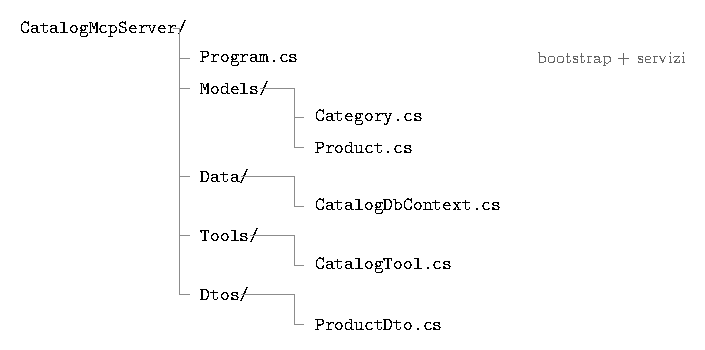
\includegraphics[keepaspectratio,alt={Struttura
consigliata del progetto
CatalogMcpServer}]{figure/struttura-progetto.pdf}}
\caption{Struttura consigliata del progetto
\protect\texttt{CatalogMcpServer}}
\end{figure}

La logica non cambia: cambia solo l'organizzazione. Nel libro teniamo
tutto insieme per leggibilità, ma nei tuoi progetti separa per
responsabilità.

\section{2.12 Il server HTTP completo}\label{il-server-http-completo}

Se il catalogo deve essere condiviso tra più utenti o macchine, il
trasporto \texttt{stdio} non basta: serve HTTP. Come nel Capitolo 1, il
passaggio è questione di pochi ritocchi.

\subsection{2.12.1 Il pacchetto
aggiuntivo}\label{il-pacchetto-aggiuntivo}

\begin{Shaded}
\begin{Highlighting}[]
\OperatorTok{\textgreater{}}\NormalTok{ dotnet }\ExtensionTok{add}\NormalTok{ package ModelContextProtocol.AspNetCore }\AttributeTok{{-}{-}version}\NormalTok{ 2.3.0}
\end{Highlighting}
\end{Shaded}

\subsection{2.12.2 Le differenze rispetto a
stdio}\label{le-differenze-rispetto-a-stdio}

Tre modifiche al codice precedente:

\begin{enumerate}
\def\labelenumi{\arabic{enumi}.}
\tightlist
\item
  \texttt{WebApplication.CreateBuilder} al posto di
  \texttt{Host.CreateApplicationBuilder};
\item
  \texttt{WithHttpTransport()} al posto di
  \texttt{WithStdioServerTransport()};
\item
  \texttt{app.MapMcp("/mcp")} per mappare l'endpoint sullo stesso
  percorso usato dai client.
\end{enumerate}

Tutto il resto --- entità, \texttt{DbContext}, tool --- resta
\textbf{identico} alla sezione 2.11: i metodi dei tool dichiarano
esplicitamente il nome pubblico, per esempio
\texttt{{[}McpServerTool(Name\ =\ "list\_products"){]}}. È la riprova
del valore del protocollo: il codice di dominio non dipende dal
trasporto.

\begin{Shaded}
\begin{Highlighting}[]
\KeywordTok{using}\NormalTok{ System}\OperatorTok{.}\FunctionTok{ComponentModel}\OperatorTok{;}
\KeywordTok{using}\NormalTok{ Microsoft}\OperatorTok{.}\FunctionTok{AspNetCore}\OperatorTok{.}\FunctionTok{Builder}\OperatorTok{;}
\KeywordTok{using}\NormalTok{ Microsoft}\OperatorTok{.}\FunctionTok{EntityFrameworkCore}\OperatorTok{;}
\KeywordTok{using}\NormalTok{ Microsoft}\OperatorTok{.}\FunctionTok{Extensions}\OperatorTok{.}\FunctionTok{DependencyInjection}\OperatorTok{;}
\KeywordTok{using}\NormalTok{ Microsoft}\OperatorTok{.}\FunctionTok{Extensions}\OperatorTok{.}\FunctionTok{Logging}\OperatorTok{;}
\KeywordTok{using}\NormalTok{ ModelContextProtocol}\OperatorTok{;}
\KeywordTok{using}\NormalTok{ ModelContextProtocol}\OperatorTok{.}\FunctionTok{Server}\OperatorTok{;}

\DataTypeTok{var}\NormalTok{ builder }\OperatorTok{=}\NormalTok{ WebApplication}\OperatorTok{.}\FunctionTok{CreateBuilder}\OperatorTok{(}\NormalTok{args}\OperatorTok{);}

\NormalTok{builder}\OperatorTok{.}\FunctionTok{Services}\OperatorTok{.}\FunctionTok{AddDbContextFactory}\OperatorTok{\textless{}}\NormalTok{CatalogDbContext}\OperatorTok{\textgreater{}(}\NormalTok{options }\OperatorTok{=\textgreater{}}
\NormalTok{    options}\OperatorTok{.}\FunctionTok{UseSqlite}\OperatorTok{(}\StringTok{"Data Source=catalog.db"}\OperatorTok{));}

\NormalTok{builder}\OperatorTok{.}\FunctionTok{Services}\OperatorTok{.}\FunctionTok{AddMcpServer}\OperatorTok{()}
    \OperatorTok{.}\FunctionTok{WithHttpTransport}\OperatorTok{()}
    \OperatorTok{.}\FunctionTok{WithTools}\OperatorTok{\textless{}}\NormalTok{CatalogTool}\OperatorTok{\textgreater{}();}

\DataTypeTok{var}\NormalTok{ app }\OperatorTok{=}\NormalTok{ builder}\OperatorTok{.}\FunctionTok{Build}\OperatorTok{();}

\CommentTok{// Inizializzazione dimostrativa, come nella versione stdio; non cancella il database.}
\OperatorTok{\{}
    \DataTypeTok{var}\NormalTok{ options }\OperatorTok{=} \KeywordTok{new}\NormalTok{ DbContextOptionsBuilder}\OperatorTok{\textless{}}\NormalTok{CatalogDbContext}\OperatorTok{\textgreater{}()}
        \OperatorTok{.}\FunctionTok{UseSqlite}\OperatorTok{(}\StringTok{"Data Source=catalog.db"}\OperatorTok{).}\FunctionTok{Options}\OperatorTok{;}
\NormalTok{    await }\KeywordTok{using} \DataTypeTok{var}\NormalTok{ seedDb }\OperatorTok{=} \KeywordTok{new} \FunctionTok{CatalogDbContext}\OperatorTok{(}\NormalTok{options}\OperatorTok{);}
\NormalTok{    await seedDb}\OperatorTok{.}\FunctionTok{Database}\OperatorTok{.}\FunctionTok{EnsureCreatedAsync}\OperatorTok{();}

    \KeywordTok{if} \OperatorTok{(!}\NormalTok{await seedDb}\OperatorTok{.}\FunctionTok{Products}\OperatorTok{.}\FunctionTok{AnyAsync}\OperatorTok{())}
    \OperatorTok{\{}
        \DataTypeTok{var}\NormalTok{ books }\OperatorTok{=}\NormalTok{ await seedDb}\OperatorTok{.}\FunctionTok{Categories}\OperatorTok{.}\FunctionTok{SingleOrDefaultAsync}\OperatorTok{(}\NormalTok{c }\OperatorTok{=\textgreater{}}\NormalTok{ c}\OperatorTok{.}\FunctionTok{Name} \OperatorTok{==} \StringTok{"Books"}\OperatorTok{)}
            \OperatorTok{??} \KeywordTok{new}\NormalTok{ Category }\OperatorTok{\{}\NormalTok{ Name }\OperatorTok{=} \StringTok{"Books"} \OperatorTok{\};}
        \DataTypeTok{var}\NormalTok{ electronics }\OperatorTok{=}\NormalTok{ await seedDb}\OperatorTok{.}\FunctionTok{Categories}\OperatorTok{.}\FunctionTok{SingleOrDefaultAsync}\OperatorTok{(}\NormalTok{c }\OperatorTok{=\textgreater{}}\NormalTok{ c}\OperatorTok{.}\FunctionTok{Name} \OperatorTok{==} \StringTok{"Electronics"}\OperatorTok{)}
            \OperatorTok{??} \KeywordTok{new}\NormalTok{ Category }\OperatorTok{\{}\NormalTok{ Name }\OperatorTok{=} \StringTok{"Electronics"} \OperatorTok{\};}
\NormalTok{        seedDb}\OperatorTok{.}\FunctionTok{Products}\OperatorTok{.}\FunctionTok{AddRange}\OperatorTok{(}
            \KeywordTok{new}\NormalTok{ Product }\OperatorTok{\{}\NormalTok{ Name }\OperatorTok{=} \StringTok{"The Lord of the Rings"}\OperatorTok{,}\NormalTok{ Price }\OperatorTok{=} \FloatTok{29.90m}\OperatorTok{,}\NormalTok{ Category }\OperatorTok{=}\NormalTok{ books }\OperatorTok{\},}
            \KeywordTok{new}\NormalTok{ Product }\OperatorTok{\{}\NormalTok{ Name }\OperatorTok{=} \StringTok{"MacBook Air"}\OperatorTok{,}\NormalTok{ Price }\OperatorTok{=} \FloatTok{1199.00m}\OperatorTok{,}\NormalTok{ Category }\OperatorTok{=}\NormalTok{ electronics }\OperatorTok{\});}
\NormalTok{        await seedDb}\OperatorTok{.}\FunctionTok{SaveChangesAsync}\OperatorTok{();}
    \OperatorTok{\}}
\OperatorTok{\}}

\NormalTok{app}\OperatorTok{.}\FunctionTok{MapMcp}\OperatorTok{(}\StringTok{"/mcp"}\OperatorTok{);}

\NormalTok{await app}\OperatorTok{.}\FunctionTok{RunAsync}\OperatorTok{();}

\CommentTok{// ... entità, DbContext e CatalogTool identici alla versione stdio ...}
\end{Highlighting}
\end{Shaded}

\subsection{2.12.3 Avviare e collegare}\label{avviare-e-collegare}

Avviamo il server su una porta:

\begin{Shaded}
\begin{Highlighting}[]
\OperatorTok{\textgreater{}}\NormalTok{ dotnet }\ExtensionTok{run} \AttributeTok{{-}{-}urls}\NormalTok{ http://localhost:5080}
\end{Highlighting}
\end{Shaded}

Il client (Claude Desktop, VS Code o l'Inspector) userà l'URL
\texttt{http://localhost:5080/mcp}. La configurazione per Claude
Desktop, per esempio:

\begin{Shaded}
\begin{Highlighting}[]
\FunctionTok{\{}
  \DataTypeTok{"mcpServers"}\FunctionTok{:} \FunctionTok{\{}
    \DataTypeTok{"catalog"}\FunctionTok{:} \FunctionTok{\{}
      \DataTypeTok{"url"}\FunctionTok{:} \StringTok{"http://localhost:5080/mcp"}
    \FunctionTok{\}}
  \FunctionTok{\}}
\FunctionTok{\}}
\end{Highlighting}
\end{Shaded}

\subsection{2.12.4 Considerazioni per il database in
HTTP}\label{considerazioni-per-il-database-in-http}

Come il listato \texttt{stdio}, anche questo è un esempio didattico, non
una configurazione di produzione. \texttt{EnsureCreated} non sostituisce
le migrazioni: per usare \texttt{dotnet\ ef}, rimuovi il blocco
dimostrativo di inizializzazione e applica le migrazioni separatamente.
Non aggiungere \texttt{EnsureDeleted} al codice eseguito all'avvio,
perché può essere eseguito anche quando gli strumenti EF Core caricano
l'app in fase di design.

Con un server HTTP condiviso, il database diventa una \textbf{risorsa
concorrente}: più richieste possono arrivare contemporaneamente. Qui il
pattern \texttt{IDbContextFactory} dà il meglio di sé: ogni richiesta
crea il proprio contesto, e SQLite (o il provider scelto) gestisce la
concorrenza a livello di file o di server. Due accortezze:

\begin{itemize}
\tightlist
\item
  per SQLite, in scenari ad alta concorrenza di scrittura, valuta di
  abilitare il \textbf{WAL} (Write-Ahead Logging) per ridurre i blocchi;
\item
  per database server (SQL Server, PostgreSQL), la concorrenza è gestita
  dal motore, e il pooling delle connessioni rende tutto fluido.
\end{itemize}

\subsection{2.12.5 Un consiglio di
architettura}\label{un-consiglio-di-architettura}

Se il catalogo deve servire sia un'applicazione tradizionale sia un
agente AI, non duplicare la logica: costruisci le tue \textbf{REST API}
per l'applicazione e un \textbf{MCP server} che usa lo stesso
\texttt{DbContext} (o gli stessi servizi applicativi) per l'agente. Come
discusso nel Capitolo 1, REST e MCP sono complementari, e condividere il
livello dati è la scelta che massimizza la coerenza e minimizza la
manutenzione.

\section{2.13 Testare il server con l'MCP
Inspector}\label{testare-il-server-con-lmcp-inspector}

Come per il Capitolo 1, l'MCP Inspector è il banco di prova ideale. Per
un server con database, però, il collaudo ha un'attenzione in più:
verificare che lo \textbf{stato} cambi correttamente tra una chiamata e
l'altra.

\subsection{2.13.1 Avviare l'Inspector}\label{avviare-linspector}

\begin{Shaded}
\begin{Highlighting}[]
\OperatorTok{\textgreater{}}\NormalTok{ npx }\ExtensionTok{@modelcontextprotocol/inspector}\NormalTok{ dotnet run }\AttributeTok{{-}{-}project}\NormalTok{ C:}\DataTypeTok{\textbackslash{}p}\NormalTok{ercorso}\DataTypeTok{\textbackslash{}C}\NormalTok{atalogMcpServer}
\end{Highlighting}
\end{Shaded}

Per la versione HTTP:

\begin{Shaded}
\begin{Highlighting}[]
\OperatorTok{\textgreater{}}\NormalTok{ npx }\ExtensionTok{@modelcontextprotocol/inspector} \AttributeTok{{-}{-}transport}\NormalTok{ http http://localhost:5080/mcp}
\end{Highlighting}
\end{Shaded}

\subsection{2.13.2 La sequenza di
collaudo}\label{la-sequenza-di-collaudo}

Esegui queste operazioni in ordine e verifica i risultati:

\begin{enumerate}
\def\labelenumi{\arabic{enumi}.}
\tightlist
\item
  \textbf{\texttt{list\_products} senza argomenti} --- deve restituire i
  due prodotti seminati all'avvio.
\item
  \textbf{\texttt{list\_products} con \texttt{\{"category":\ "Books"\}}}
  --- deve restituire solo il prodotto della categoria ``Books''.
\item
  \textbf{\texttt{search\_products} con \texttt{\{"term":\ "Mac"\}}} ---
  deve trovare ``MacBook Air''.
\item
  \textbf{\texttt{create\_product}} con
  \texttt{\{"name":\ "Headphones",\ "price":\ 199.99,\ "categoryName":\ "Electronics"\}}
  --- deve creare il prodotto e restituire l'id.
\item
  \textbf{\texttt{list\_products} di nuovo} --- deve ora mostrare il
  nuovo prodotto: questo conferma che il \textbf{database persiste} le
  modifiche.
\item
  \textbf{\texttt{delete\_product}} con l'id del prodotto appena creato
  --- deve eliminarlo.
\item
  \textbf{\texttt{create\_product} con una categoria inesistente} ---
  deve restituire l'errore \texttt{Category\ not\ found:\ ...}, non un
  crash.
\item
  \textbf{\texttt{delete\_product} con un id inesistente} --- deve
  restituire \texttt{Product\ not\ found:\ ...}.
\end{enumerate}

\subsection{2.13.3 Cosa osservare negli
errori}\label{cosa-osservare-negli-errori}

Una \texttt{McpException} lanciata dal tool non è un errore di
protocollo JSON-RPC: \texttt{tools/call} restituisce normalmente un
risultato con \texttt{isError:\ true} e il messaggio in
\texttt{content}, per esempio:

\begin{Shaded}
\begin{Highlighting}[]
\FunctionTok{\{}
  \DataTypeTok{"jsonrpc"}\FunctionTok{:} \StringTok{"2.0"}\FunctionTok{,}
  \DataTypeTok{"id"}\FunctionTok{:} \DecValTok{1}\FunctionTok{,}
  \DataTypeTok{"result"}\FunctionTok{:} \FunctionTok{\{}
    \DataTypeTok{"content"}\FunctionTok{:} \OtherTok{[}\FunctionTok{\{} \DataTypeTok{"type"}\FunctionTok{:} \StringTok{"text"}\FunctionTok{,} \DataTypeTok{"text"}\FunctionTok{:} \StringTok{"Product not found: 999"} \FunctionTok{\}}\OtherTok{]}\FunctionTok{,}
    \DataTypeTok{"isError"}\FunctionTok{:} \KeywordTok{true}
  \FunctionTok{\}}
\FunctionTok{\}}
\end{Highlighting}
\end{Shaded}

Il campo JSON-RPC di primo livello \texttt{error} è invece riservato
agli errori di protocollo, per esempio una richiesta non valida o un
metodo sconosciuto. Verifica che il risultato del tool sia
\textbf{chiaro e contestualizzato}, non un generico ``internal error'':
se il modello riceve un errore chiaro, può correggersi; se riceve un
errore opaco, fallisce e frustra l'utente.

\subsection{2.13.4 Testare la persistenza attraverso il
riavvio}\label{testare-la-persistenza-attraverso-il-riavvio}

Un test che vale la pena fare: crea un prodotto, \textbf{chiudi
l'Inspector} (che termina il server), riavvia il server e verifica con
\texttt{list\_products} che il prodotto esista ancora.
L'inizializzazione dimostrativa usa \texttt{EnsureCreated} senza
cancellare il database e semina i prodotti solo se non ce ne sono: il
prodotto creato deve quindi persistere al riavvio. È comunque un
artificio didattico, non una strategia di inizializzazione per la
produzione.

\subsection{2.13.5 Test automatici con un client
.NET}\label{test-automatici-con-un-client-.net}

Nel Capitolo 1 abbiamo visto come scrivere un client .NET. Lo stesso
approccio si applica qui e diventa un \textbf{test di integrazione}
prezioso: avvia il server, invoca \texttt{create\_product}, poi
\texttt{list\_products}, e verifica che il nuovo prodotto compaia. Il
pattern è identico a quello già mostrato; la differenza è che ora,
dietro i tool, c'è un database reale.

\section{2.14 Primitivi avanzati: il
Progress}\label{primitivi-avanzati-il-progress}

Finora i nostri tool sono ``tutto o niente'': partono, lavorano e
restituiscono un risultato. Ma un'operazione lunga --- per esempio una
query pesante, un'importazione o un calcolo --- trae beneficio dal
\textbf{reporting del progresso}: il server informa il client di quanto
manca al completamento, e il client può mostrarlo all'utente.

\subsection{2.14.1 Il meccanismo}\label{il-meccanismo}

MCP prevede che il client, quando invoca un tool, possa allegare un
\textbf{progress token}. Il server, durante l'esecuzione, invia
notifiche \texttt{notifications/progress} con quel token, comunicando
una frazione di avanzamento (0..1), un totale opzionale e un messaggio.

L'SDK .NET rende tutto questo trasparente: basta dichiarare nel tool un
parametro di tipo
\textbf{\texttt{IProgress\textless{}ProgressNotificationValue\textgreater{}}}.
L'SDK lo riconosce come parametro speciale, lo \textbf{esclude dallo
schema di input} e lo inietta automaticamente, collegato al progress
token del client.

\subsection{2.14.2 Un tool con progress}\label{un-tool-con-progress}

Estendiamo il nostro catalogo con un tool che conta i prodotti simulando
un lavoro lungo:

\begin{Shaded}
\begin{Highlighting}[]
\KeywordTok{using}\NormalTok{ ModelContextProtocol}\OperatorTok{.}\FunctionTok{Protocol}\OperatorTok{;}

\OperatorTok{[}\NormalTok{McpServerTool}\OperatorTok{,} \FunctionTok{Description}\OperatorTok{(}\StringTok{"Counts products, reporting progress while working."}\OperatorTok{)]}
\KeywordTok{public}\NormalTok{ async Task}\OperatorTok{\textless{}}\DataTypeTok{string}\OperatorTok{\textgreater{}} \FunctionTok{CountWithProgress}\OperatorTok{(}
\NormalTok{    IProgress}\OperatorTok{\textless{}}\NormalTok{ProgressNotificationValue}\OperatorTok{\textgreater{}?}\NormalTok{ progress }\OperatorTok{=} \KeywordTok{null}\OperatorTok{,}
\NormalTok{    CancellationToken cancellationToken }\OperatorTok{=} \KeywordTok{default}\OperatorTok{)}
\OperatorTok{\{}
\NormalTok{    await }\KeywordTok{using} \DataTypeTok{var}\NormalTok{ db }\OperatorTok{=}\NormalTok{ await factory}\OperatorTok{.}\FunctionTok{CreateDbContextAsync}\OperatorTok{(}\NormalTok{cancellationToken}\OperatorTok{);}

\NormalTok{    progress}\OperatorTok{?.}\FunctionTok{Report}\OperatorTok{(}\KeywordTok{new}\NormalTok{ ProgressNotificationValue}
    \OperatorTok{\{}
\NormalTok{        Progress }\OperatorTok{=} \FloatTok{0.2f}\OperatorTok{,}
\NormalTok{        Total }\OperatorTok{=} \DecValTok{1}\NormalTok{f}\OperatorTok{,}
\NormalTok{        Message }\OperatorTok{=} \StringTok{"querying the database"}
    \OperatorTok{\});}

    \DataTypeTok{var}\NormalTok{ total }\OperatorTok{=}\NormalTok{ await db}\OperatorTok{.}\FunctionTok{Products}\OperatorTok{.}\FunctionTok{CountAsync}\OperatorTok{(}\NormalTok{cancellationToken}\OperatorTok{);}

\NormalTok{    progress}\OperatorTok{?.}\FunctionTok{Report}\OperatorTok{(}\KeywordTok{new}\NormalTok{ ProgressNotificationValue}
    \OperatorTok{\{}
\NormalTok{        Progress }\OperatorTok{=} \DecValTok{1}\NormalTok{f}\OperatorTok{,}
\NormalTok{        Total }\OperatorTok{=} \DecValTok{1}\NormalTok{f}\OperatorTok{,}
\NormalTok{        Message }\OperatorTok{=} \StringTok{"done"}
    \OperatorTok{\});}

    \KeywordTok{return}\NormalTok{ $}\StringTok{"counted \{total\} products"}\OperatorTok{;}
\OperatorTok{\}}
\end{Highlighting}
\end{Shaded}

Osservazioni:

\begin{itemize}
\tightlist
\item
  \texttt{Progress} e \texttt{Total} sono di tipo \texttt{float}: da qui
  i suffissi \texttt{f} sui letterali.
\item
  Il parametro è opzionale (\texttt{?\ progress\ =\ null}): se il client
  non fornisce un progress token, l'SDK passa \texttt{null} e il tool
  funziona comunque.
\item
  Lo schema di input del tool resta \textbf{vuoto}
  (\texttt{\{"type":"object","properties":\{\}\}}): \texttt{IProgress}
  non è un argomento, è un canale.
\end{itemize}

\subsection{2.14.3 Perché è utile}\label{perchuxe9-uxe8-utile}

In un tool che importa migliaia di righe o interroga più sistemi, il
progress trasforma un'attesa cieca in un'esperienza informata: l'host
può mostrare una barra o un messaggio, e il modello può decidere se
attendere o suggerire alternative. È un primitivo semplice ma che
aumenta molto la percezione di affidabilità di un agente.

\subsection{2.14.4 Una nota sul token}\label{una-nota-sul-token}

Non devi gestire il token a mano: l'SDK associa il parametro
\texttt{IProgress} al token della richiesta corrente. Se più invocazioni
avvengono in parallelo, ogni tool ha il suo canale di progress isolato.
È l'ennesimo caso in cui l'SDK trasforma una complessità di protocollo
in un semplice costrutto C\#.

\section{2.15 Riepilogo, glossario ed
esercizi}\label{riepilogo-glossario-ed-esercizi}

Abbiamo trasformato il catalogo MCP senza stato del Capitolo 1 in un
servizio che consulta e modifica dati persistenti. Ripercorriamo le
scelte principali e usiamole come base per la pratica.

\subsection{2.15.1 Riepilogo}\label{riepilogo}

\begin{itemize}
\tightlist
\item
  Entity Framework Core traduce le query LINQ in operazioni sul
  database; \texttt{Select} definisce i dati restituiti e spesso rende
  superfluo \texttt{Include}.
\item
  Un \texttt{DbContext} non va condiviso tra invocazioni concorrenti:
  \texttt{IDbContextFactory\textless{}TContext\textgreater{}} permette
  di creare un contesto per ogni chiamata del tool.
\item
  I DTO limitano i dati esposti al modello e separano il contratto MCP
  dalle entità persistite.
\item
  Gli input del modello vanno convalidati come qualsiasi altro input
  esterno; le scritture e le operazioni distruttive richiedono
  particolare cautela.
\item
  \texttt{EnsureCreated} e la semina idempotente sono comodi per una
  demo, ma non sostituiscono le migrazioni né una strategia di
  deployment.
\item
  \texttt{stdio} e Streamable HTTP cambiano il trasporto, non il
  contratto dei tool; Progress comunica l'avanzamento quando
  un'operazione richiede tempo.
\end{itemize}

\subsection{2.15.2 Glossario}\label{glossario}

{\def\LTcaptype{none} % do not increment counter
\begin{longtable}[]{@{}
  >{\raggedright\arraybackslash}p{(\linewidth - 2\tabcolsep) * \real{0.5000}}
  >{\raggedright\arraybackslash}p{(\linewidth - 2\tabcolsep) * \real{0.5000}}@{}}
\toprule\noalign{}
\begin{minipage}[b]{\linewidth}\raggedright
Termine
\end{minipage} & \begin{minipage}[b]{\linewidth}\raggedright
Significato
\end{minipage} \\
\midrule\noalign{}
\endhead
\bottomrule\noalign{}
\endlastfoot
\textbf{ORM} & Libreria che mappa oggetti e relazioni alle strutture di
un database. \\
\textbf{DbContext} & Unità di lavoro EF Core che gestisce query,
tracking e salvataggi. \\
\textbf{DTO} & Oggetto che definisce i dati scambiati attraverso un
contratto esterno. \\
\textbf{Migration} & Modifica versionata dello schema del database,
applicabile in modo controllato. \\
\textbf{Progress token} & Token fornito dal client per correlare le
notifiche di avanzamento di una richiesta. \\
\end{longtable}
}

\subsection{2.15.3 Esercizi proposti}\label{esercizi-proposti}

\begin{enumerate}
\def\labelenumi{\arabic{enumi}.}
\tightlist
\item
  Estendi \texttt{list\_products} con un intervallo di prezzo opzionale
  e verifica che il filtro venga eseguito dal database.
\item
  Scrivi un test d'integrazione per \texttt{delete\_product} e verifica
  che il client possa rilevare l'annotazione distruttiva.
\item
  Scrivi un test d'integrazione per la ricerca per nome e specifica il
  comportamento atteso quando il termine è vuoto.
\item
  Aggiungi una migration e prova ad applicarla a un database di sviluppo
  senza cancellare i dati esistenti.
\item
  Estendi il tool con Progress per un'importazione simulata; gestisci la
  cancellazione e comunica solo avanzamenti significativi.
\end{enumerate}

\backmatter
\end{document}
